% Updated by Michael Gertz, April 2017
%%%%%%%%%%%%%%%%%%%%%%%%%%%%

\documentclass{beamer}
%\usepackage[ngerman]{babel}
\usepackage[utf8]{inputenc}

\usepackage{color}
\usepackage{graphicx}
\usepackage{fancybox}

\usepackage{caption}

\usepackage{booktabs}

\usepackage{beamerthemesplit}
\usetheme[compress]{Heidelberg}
\definecolor{unirot}{rgb}{0.5976525,0,0}
\usecolortheme[named=unirot]{structure}


\title[Building Conversational QA-Systems]{Building Conversational \newline Question Answering Systems}
\subtitle{Master's Thesis Presentation}
\author[Stephan Lenert]{Stephan Lenert}
% \date{\today}
\date{April 16, 2024}
\institute[Uni HD]{
Heidelberg University\\
Institute of Computer Science\\
Data Science\\
\color{unirot}{stephan.lenert@stud.uni-heidelberg.de}}

%---------------------------------------%
%---------- RECURRING OUTLINE ----------%
% have this if you'd like a recurring outline
\AtBeginSection[]  % "Beamer, do the following at the start of every section"
{
\begin{frame}<beamer> 
\frametitle{Outline} % make a frame titled "Outline"
\tableofcontents[currentsection,hideallsubsections]  % show TOC and highlight current section
\end{frame}
}
%----------------------------------------


\begin{document}
\frame[plain]{\titlepage}
\frame{\frametitle{Outline}\tableofcontents[hideallsubsections]}

%========================================
%========================================

\section[Introduction]{Introduction}

\subsection{Introduction}

\frame{
\frametitle{Introduction}

  \begin{overprint}
  \onslide<1>
  \begin{figure}
  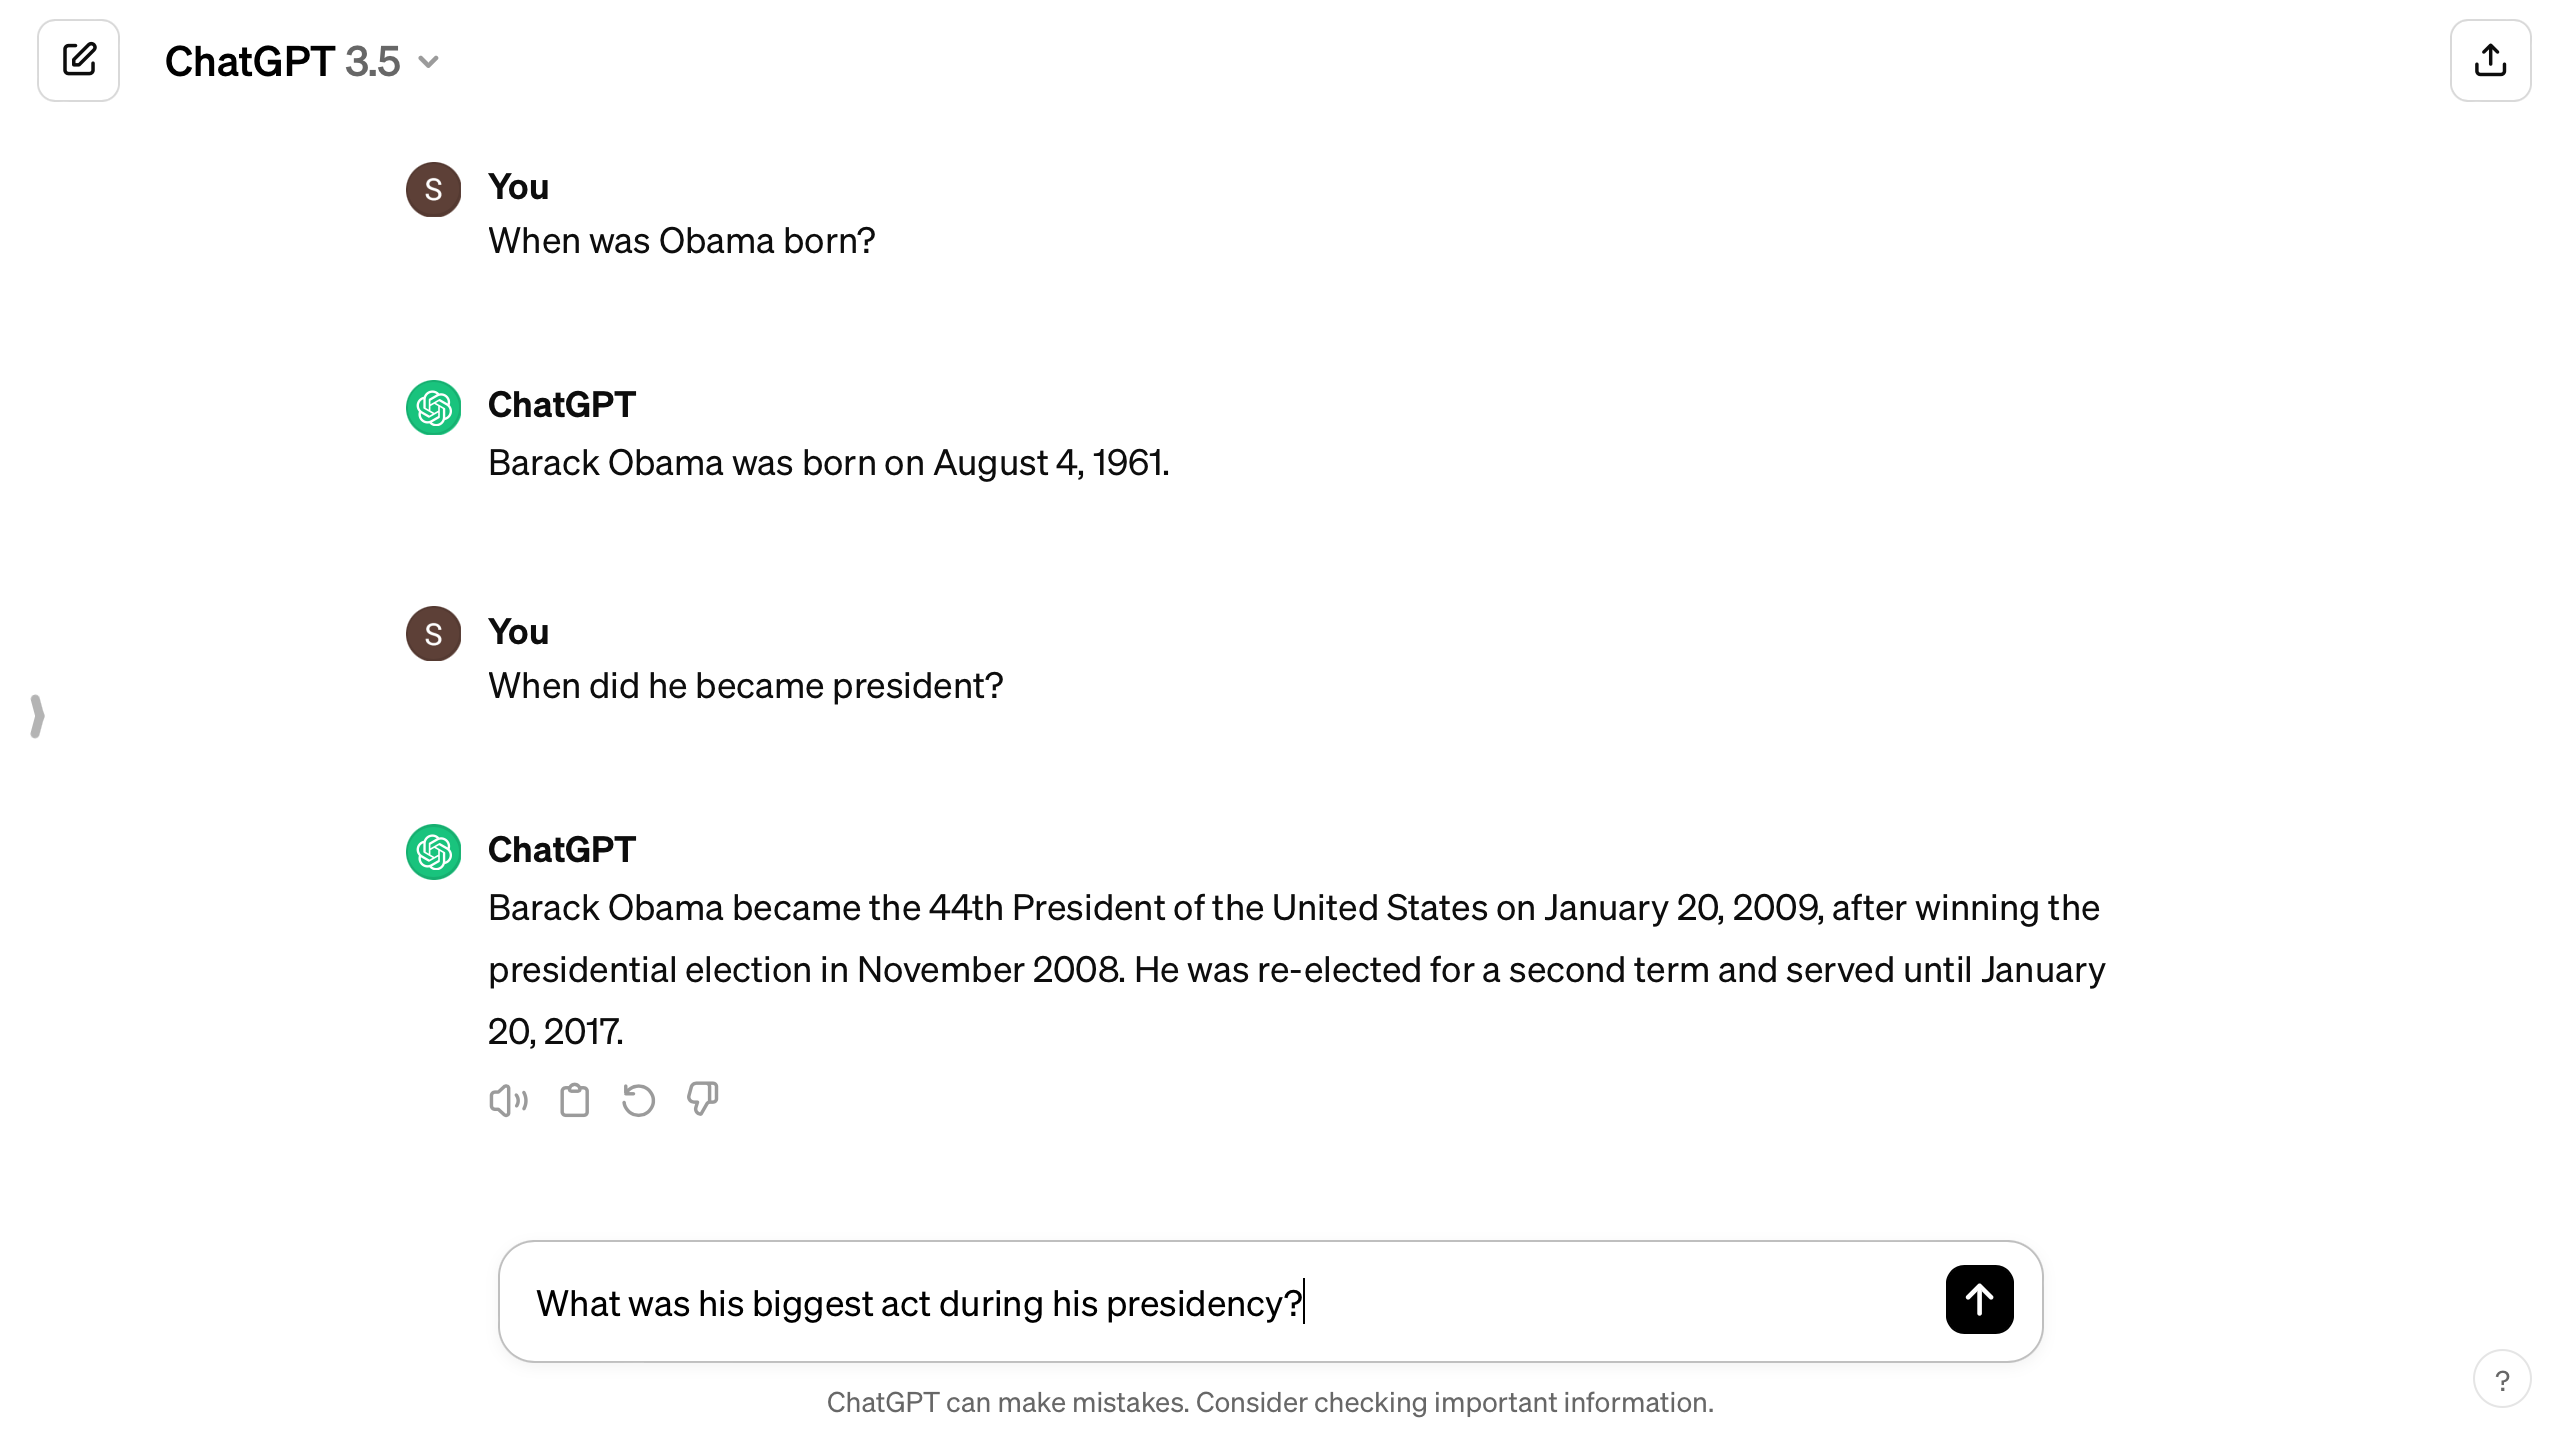
\includegraphics[width=\textwidth]{Grafiken/Obama_Chatgpt.png} 
  \captionsetup{font={tiny}} % This line changes the caption font size
  \caption{Question Answering with ChatGPT, \textit{Source: chat.openai.com}}
  \end{figure}
  \onslide<2>
  \begin{figure}
  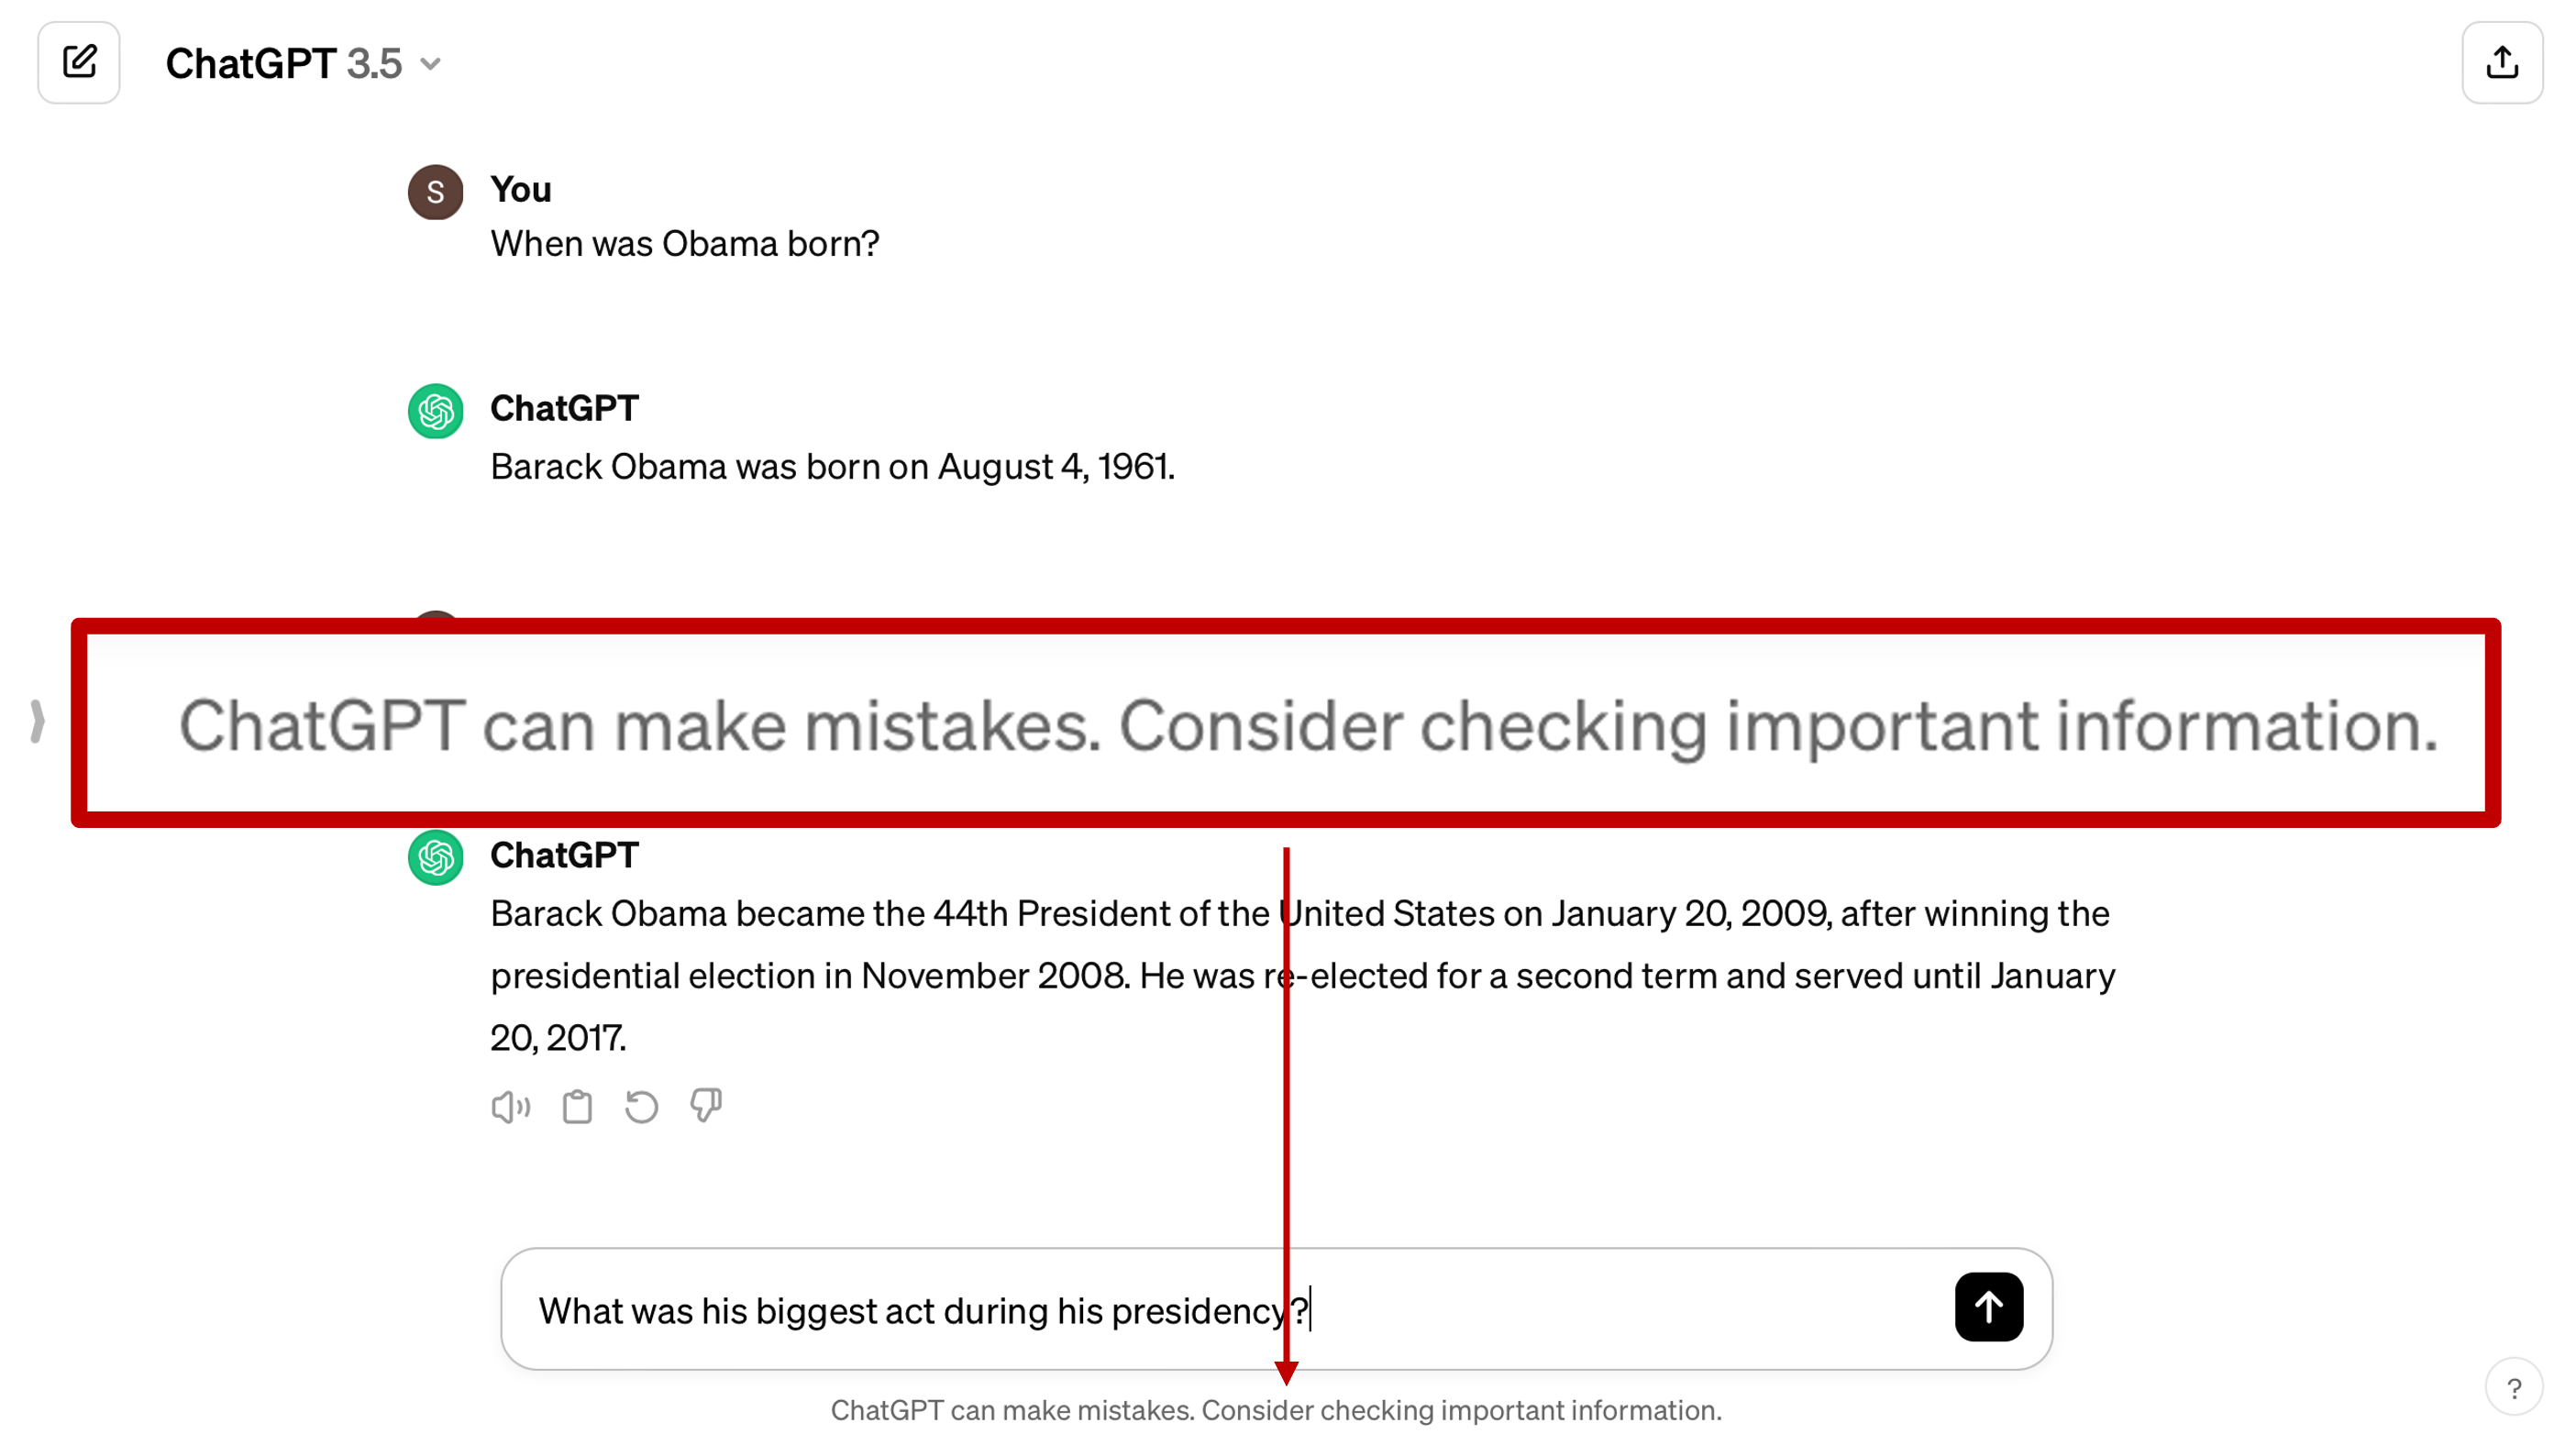
\includegraphics[width=\textwidth]{Grafiken/Chatgpt_Message_Highlight.png}
  \captionsetup{font={tiny}} % This line changes the caption font size
  \caption{Question Answering with ChatGPT, \textit{Source: chat.openai.com}}
  \end{figure}
  \end{overprint}

}

\frame{
\frametitle{Generative-only QA-Systems}

  {\color{unirot}Issues of generative-only Question Answering (QA)-systems:}
  \begin{itemize}
    \item Parameterized Knowledge
    \item Explainability
    \item Hallucination
  \end{itemize}

% Mention Source
  \bigskip
  \textbf{Source:} [Lewis et al., 2020b]  
  \bigskip
}

\frame{
  \frametitle{How to build Use-Case specific QA-Systems?}
  % Three Rows

  \begin{overprint}
  \onslide<1>

    \begin{table}
      \renewcommand{\arraystretch}{1.5} % Add more vertical spacing to the table
      \resizebox{\textwidth}{!}{%
      \begin{tabular}{|l|l|l|l|}
      \hline
      \textbf{Author/Organisation} & \textbf{Type} & \textbf{Publication Date} & \textbf{Drawbacks} \\ \hline
      Song Feng & Research Paper & 2021 & \begin{tabular}[c]{@{}l@{}}- Uses visual QA methods\\- Not latest LLMs\end{tabular} \\ \hline
      Langchain & Opensource Project & 2023 & \begin{tabular}[c]{@{}l@{}}- Bound to explicit RAG\\- Limited tool options \end{tabular}\\ \hline
      OpenAI Plugins & \begin{tabular}[c]{@{}l@{}}Commercial Tool\\ + Opensource Repository\end{tabular} & 2023 & \begin{tabular}[c]{@{}l@{}}- Same as Langchain\\- Limited to ChatGPT\end{tabular} \\ \hline
      \end{tabular}%
      }
      \captionsetup{font={tiny}} % This line changes the caption font size
      \caption{Sources for building a holistic use-case specific QA-system}
      \label{tab:sources}
    \end{table}

    \vfill
  \onslide<2>
        
    \begin{table}
      \renewcommand{\arraystretch}{1.5} % Add more vertical spacing to the table
      \resizebox{\textwidth}{!}{%
      \begin{tabular}{|l|l|l|l|}
      \hline
      \textbf{Author/Organisation} & \textbf{Type} & \textbf{Publication Date} & \textbf{Drawbacks} \\ \hline
      Song Feng & Research Paper & 2021 & \begin{tabular}[c]{@{}l@{}}- Uses visual QA methods\\- Not latest LLMs\end{tabular} \\ \hline
      Langchain & Opensource Project & 2023 & \begin{tabular}[c]{@{}l@{}}- Bound to explicit RAG\\- Limited tool options \end{tabular}\\ \hline
      OpenAI Plugins & \begin{tabular}[c]{@{}l@{}}Commercial Tool\\ + Opensource Repository\end{tabular} & 2023 & \begin{tabular}[c]{@{}l@{}}- Same as Langchain\\- Limited to ChatGPT\end{tabular} \\ \hline
      \end{tabular}%
      }
      \captionsetup{font={tiny}} % This line changes the caption font size
      \caption{Sources for building a holistic use-case specific QA-system}
      \label{tab:sources}
    \end{table}

    \vfill

    \begin{block}{There exists a Research Gap ...}
    No research work explores the use-case specific implementation of conversational question answering systems.
    \end{block}

  \end{overprint}
}

\frame{
\frametitle{Example Use-Case}

\begin{overprint}
\onslide<1>
\begin{figure}
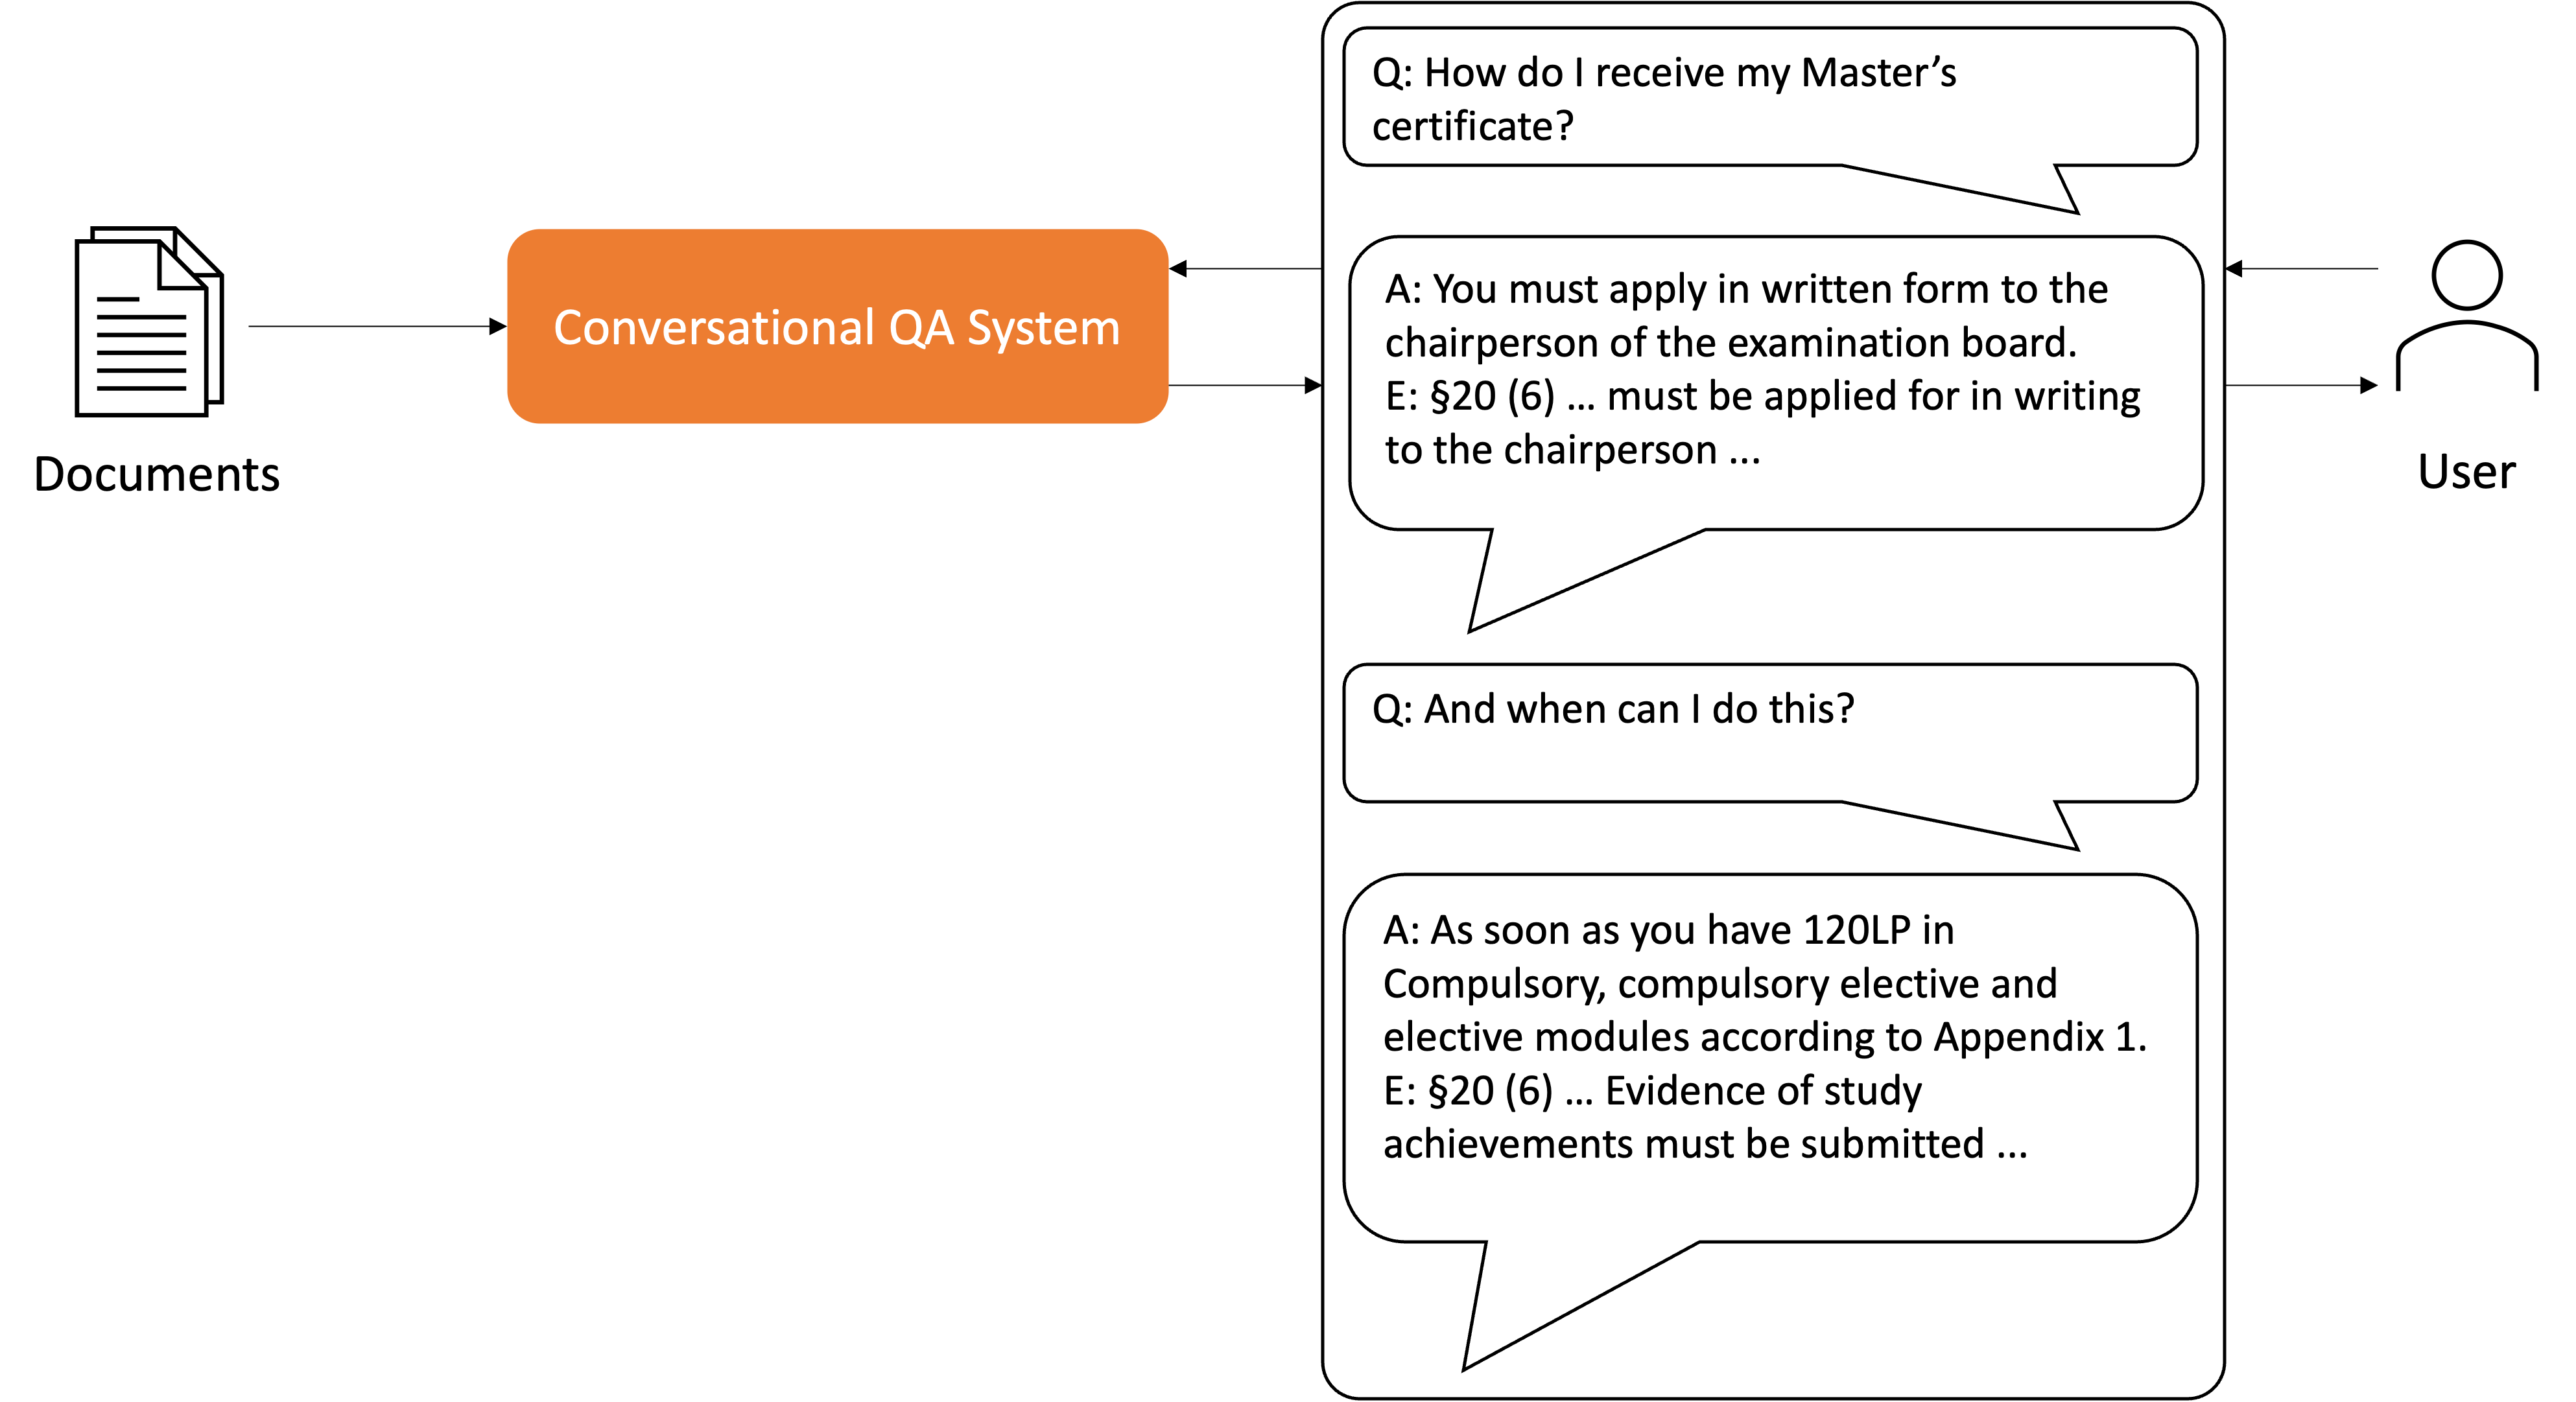
\includegraphics[width=\textwidth]{Grafiken/Use_Case.png}
\captionsetup{font={tiny}} % This line changes the caption font size
\caption{Overview of the Example Use-Case}
\end{figure}

\onslide<2>
\begin{figure}
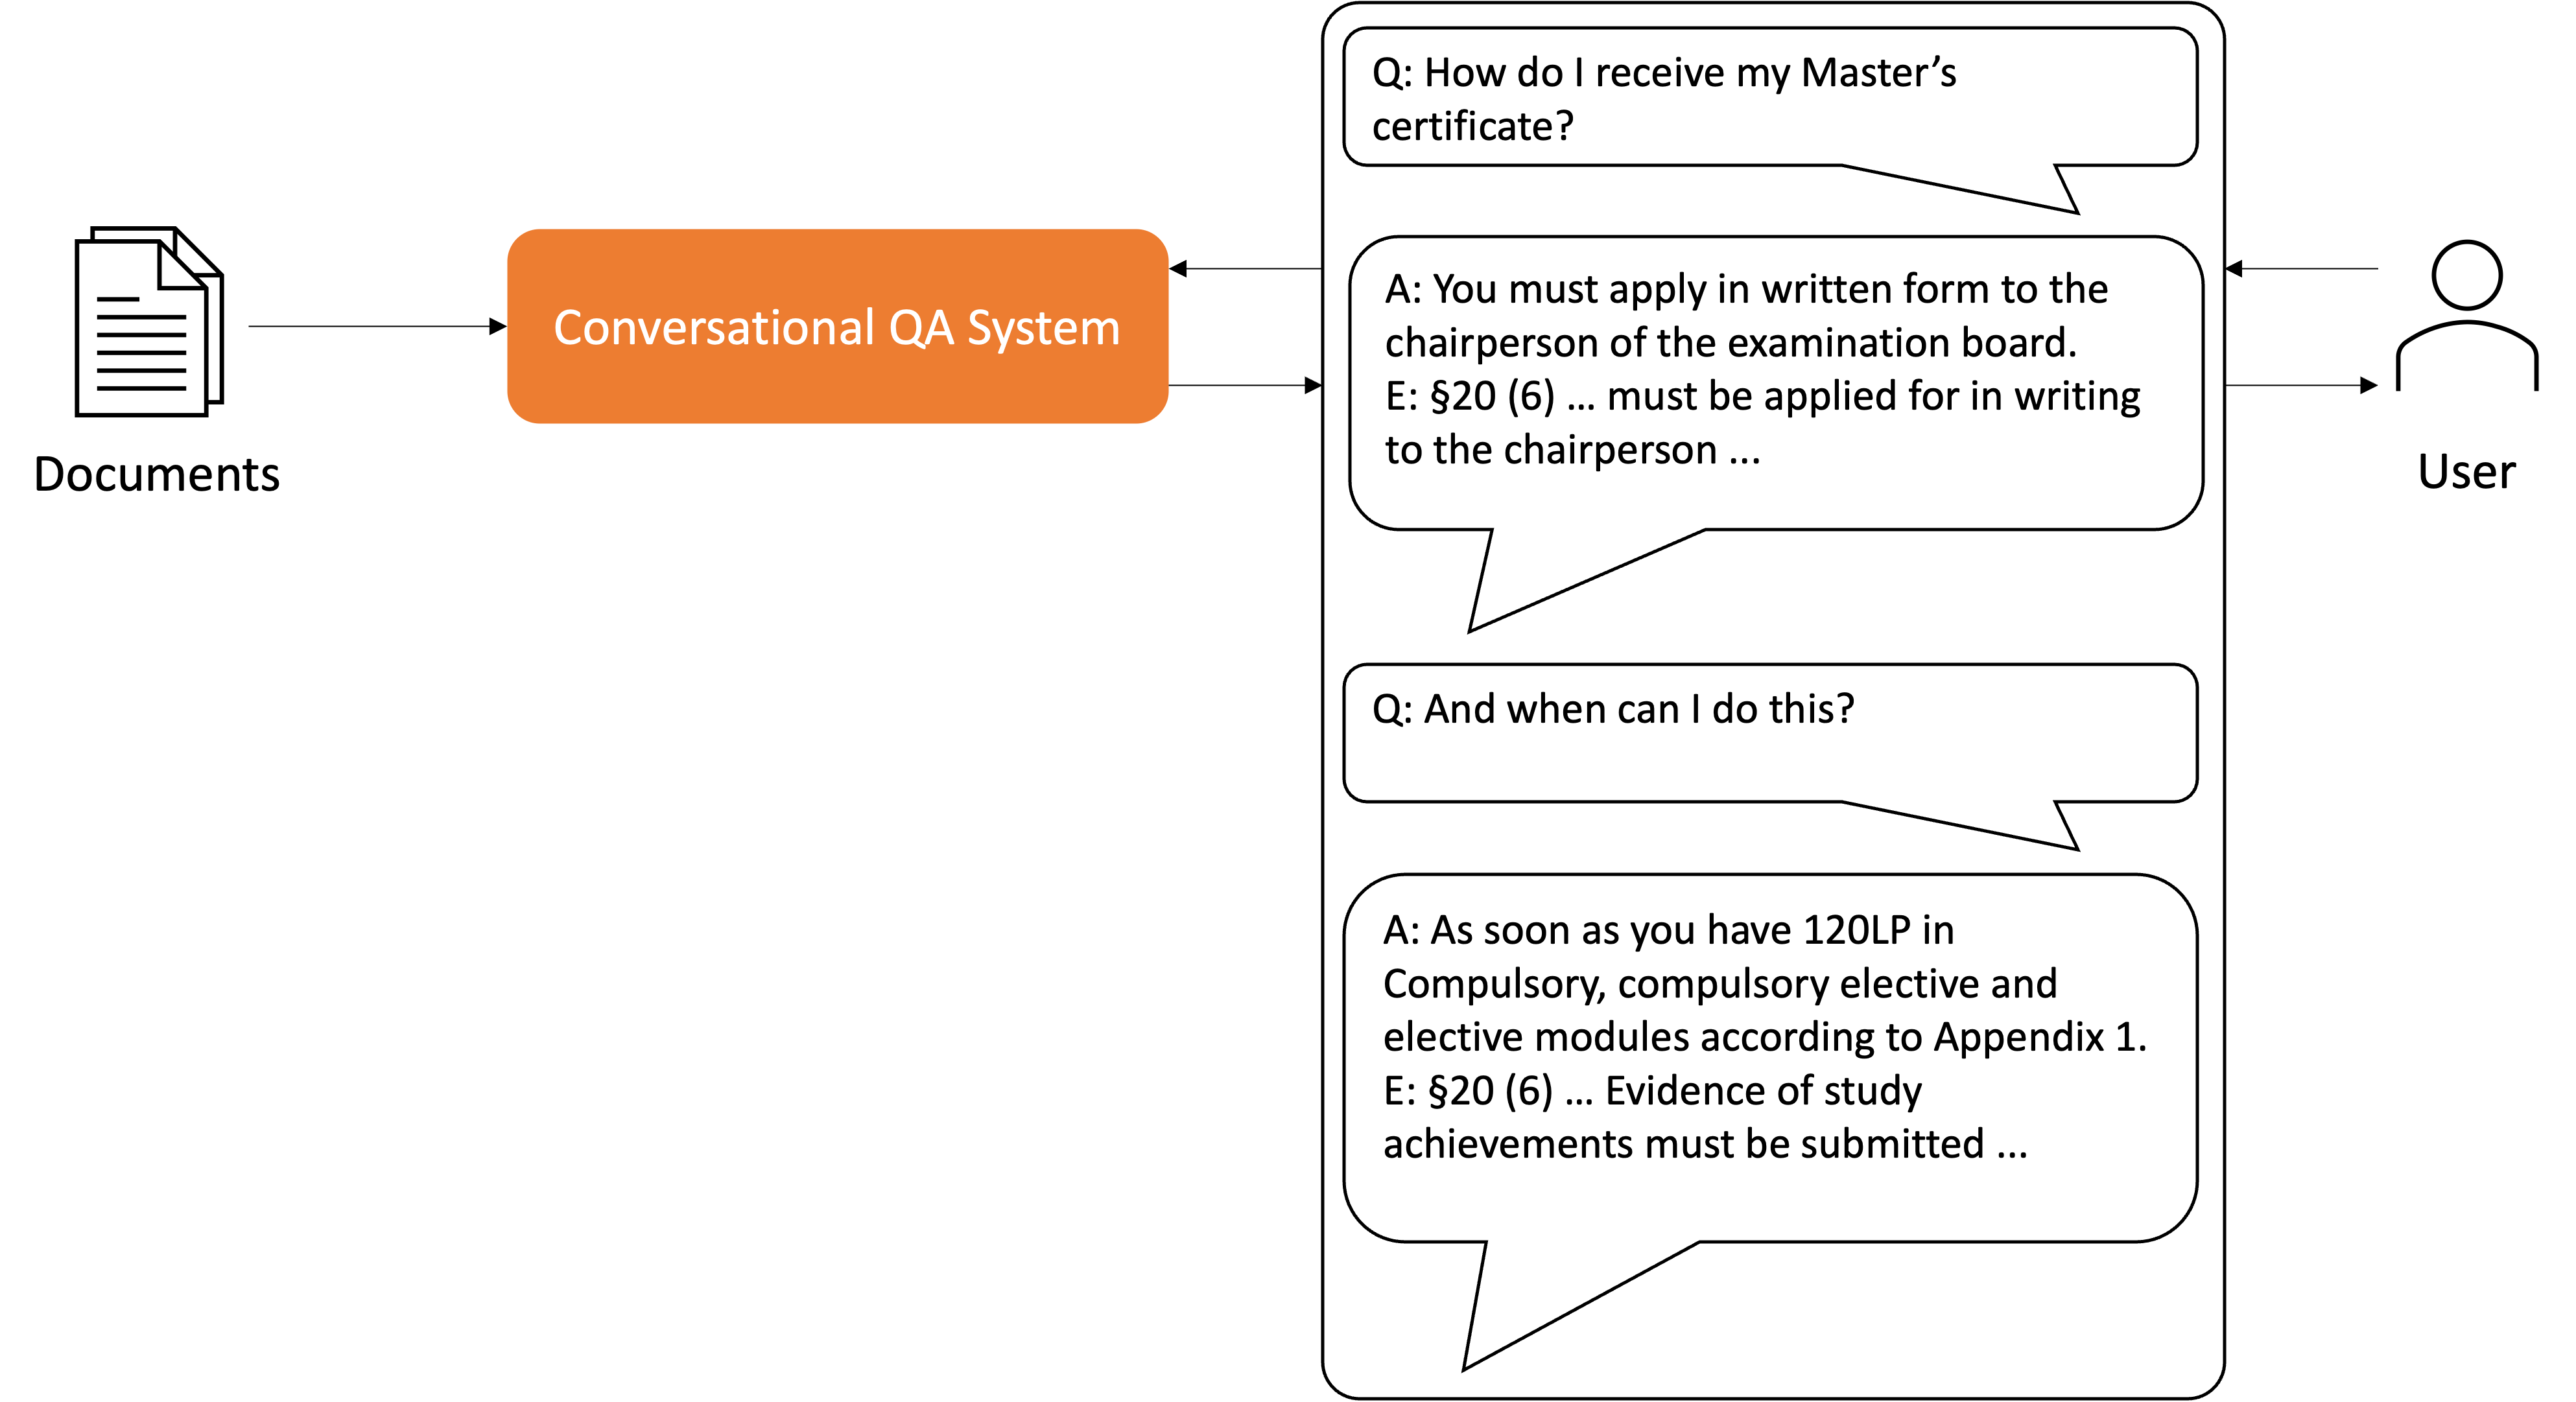
\includegraphics[width=\textwidth]{Grafiken/Use_Case.png}
\captionsetup{font={tiny}} % This line changes the caption font size
\caption{Overview of the Example Use-Case}
\end{figure}
\vspace*{-5cm}
\begin{block}{Defined Goal}
  Build a framework for a conversational question-answering system that is tailored to a specific collection of documents.
\end{block}
\end{overprint}
}

% \section[Thesis' Goal]{Goal of the Thesis}


\section[Fundamentals]{Fundamental Concepts}

\begin{frame}
  \frametitle{Natural Language QA}

  \begin{figure}
    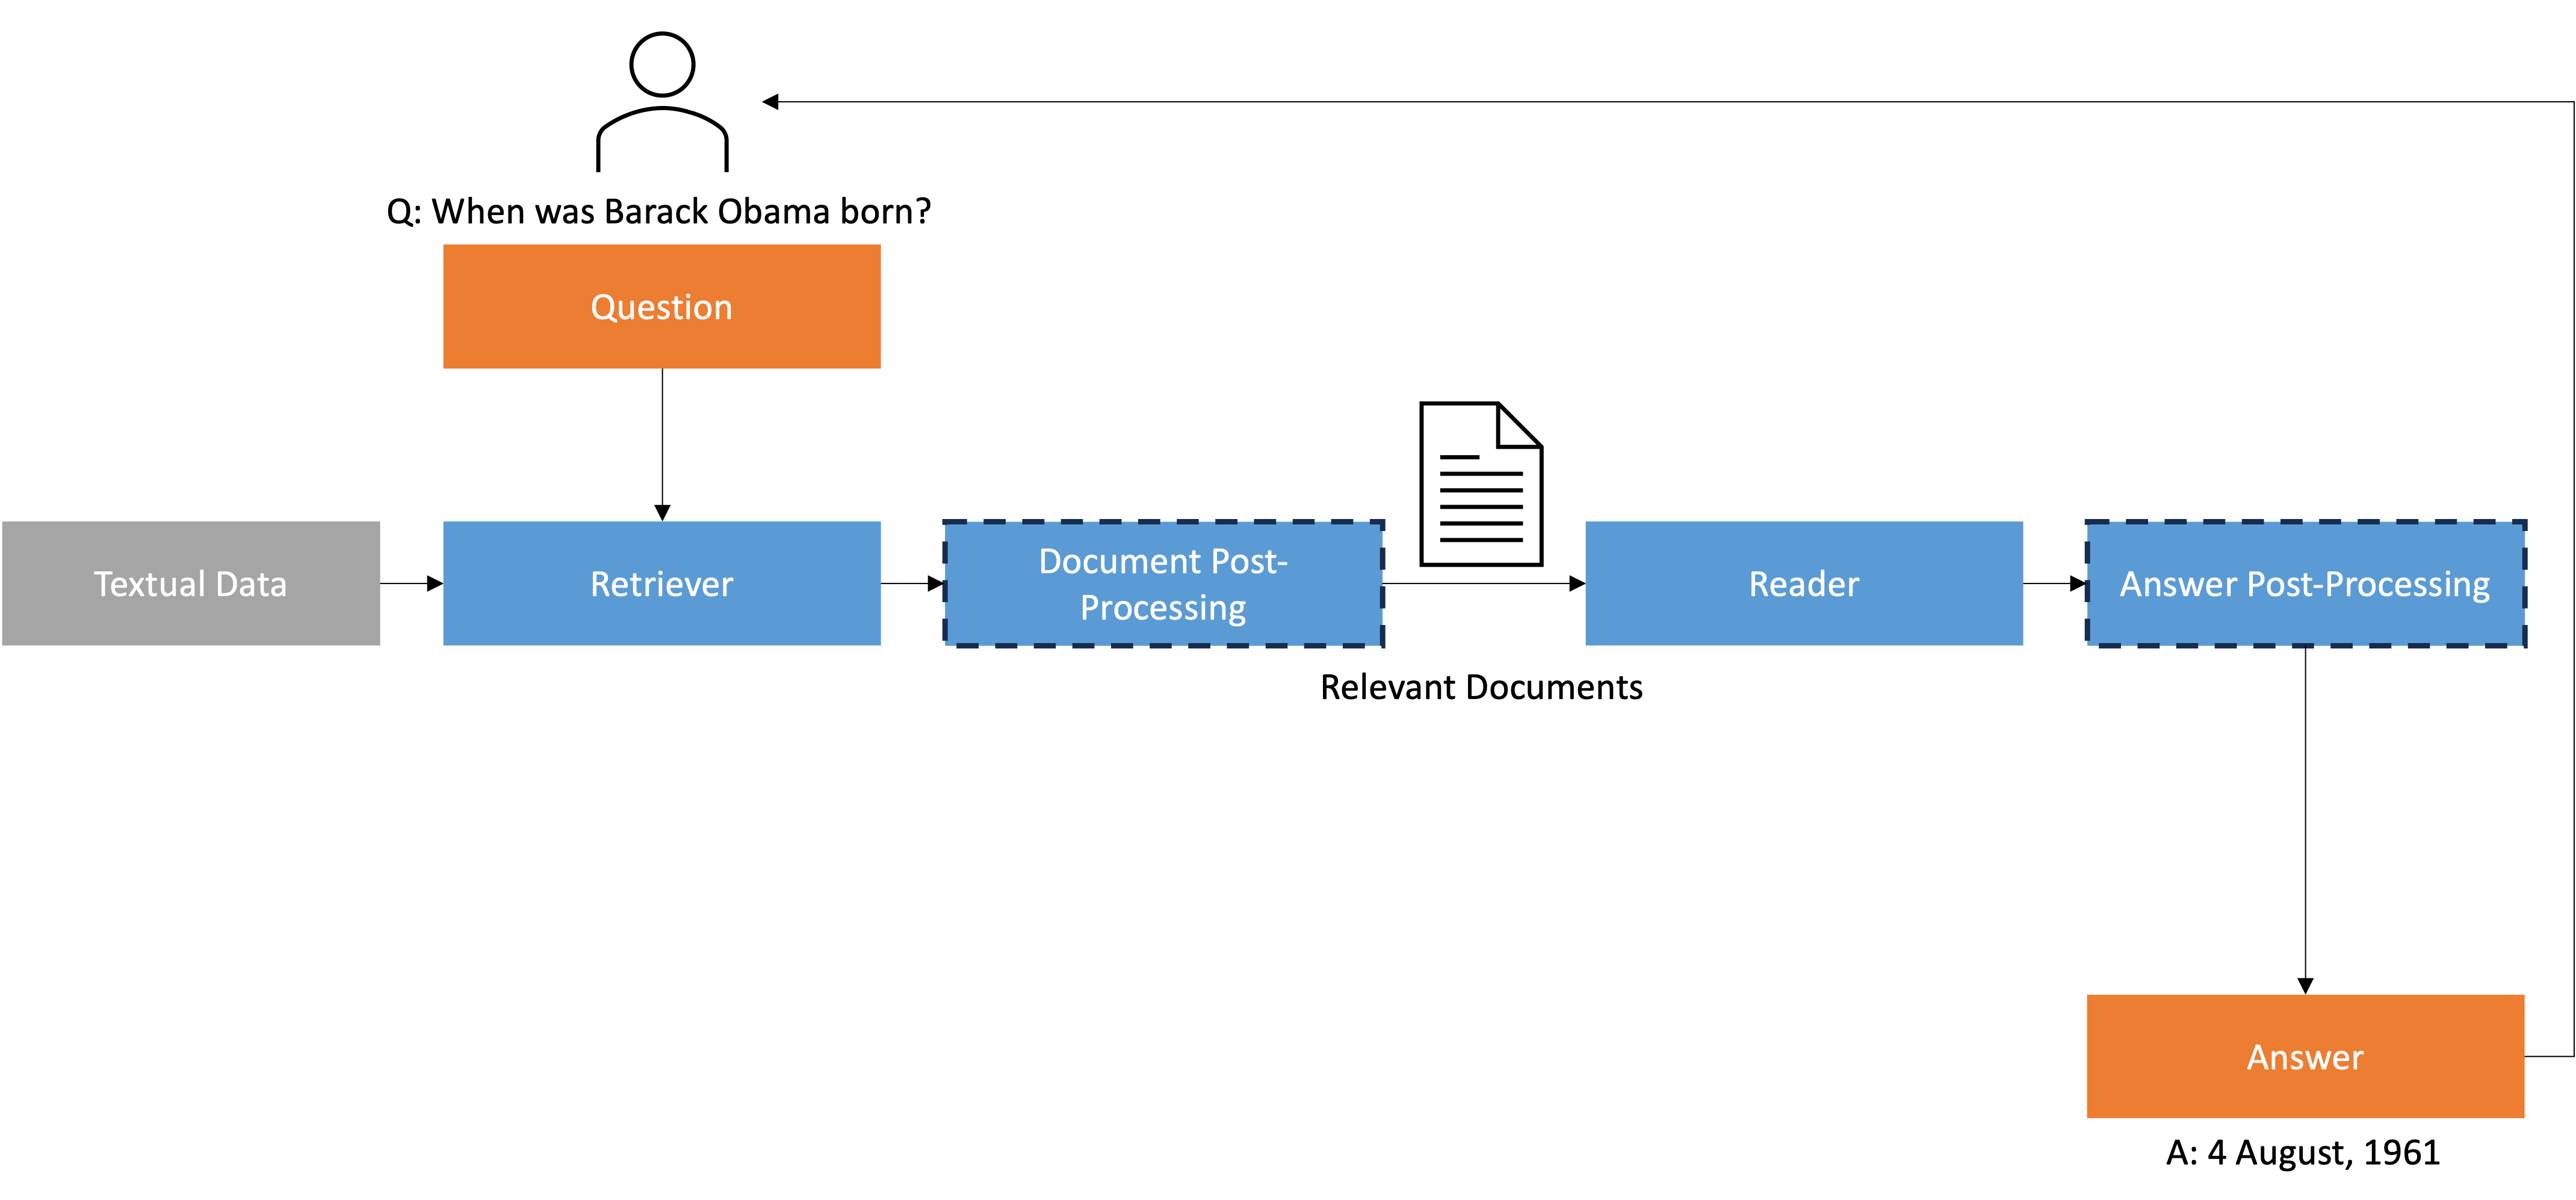
\includegraphics[width=\textwidth]{Grafiken/Retriever_Reader.png}
    \captionsetup{font={tiny}} % This line changes the caption font size
    \caption{Reader-Retriever-System Architecture for QA by Zhu et al. [Zhu et al., 2021]}
  \end{figure}

\end{frame}

\begin{frame}
  \frametitle{Retriever and Reader}

  % Create two rows retriever and reader
  \begin{columns}[t]
    \begin{column}{.5\textwidth}
    {\color{unirot}Retriever}
    \begin{itemize}
      \item Retrieves relevant documents given a query
      \item Existing approaches
      \begin{itemize}
        \item Sparse Retrieval
        \item Dense Retrieval
        \item Iterative Retrieval
      \end{itemize}
    \end{itemize}
    \end{column}
    \begin{column}{.5\textwidth}
    {\color{unirot}Reader}
    \begin{itemize}
      \item Extracts answers from evidence set given a query
      \item Existing approaches
      \begin{itemize}
        \item Extractive
        \item Generative
      \end{itemize}
    \end{itemize}
    \end{column}
  \end{columns}

\end{frame}

\begin{frame}
  \frametitle{Retrieval-Augmented Generation}

  \begin{figure}
    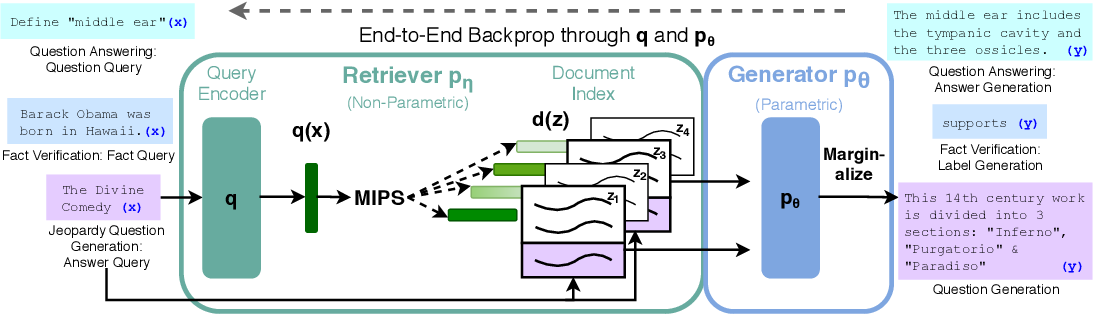
\includegraphics[width=\textwidth]{Grafiken/RAG-Figure1.png}
    \captionsetup{font={tiny}} % This line changes the caption font size
    \caption{RAG by Lewis et al. [Lewis et al., 2020b]}
  \end{figure}

  RAG:
  \begin{itemize}
    \item Extends parametric knowledge of generator by non-parametric retrieved evidences
    \item Originally proposed as end-to-end training
    \item Modern RAG implementations use explicit evidence sets
  \end{itemize}
  
\end{frame}

\begin{frame}{Conversation}
  
  \begin{columns}[t] % align columns
    \begin{column}{.6\textwidth}
      \vfill
      \begin{figure}
        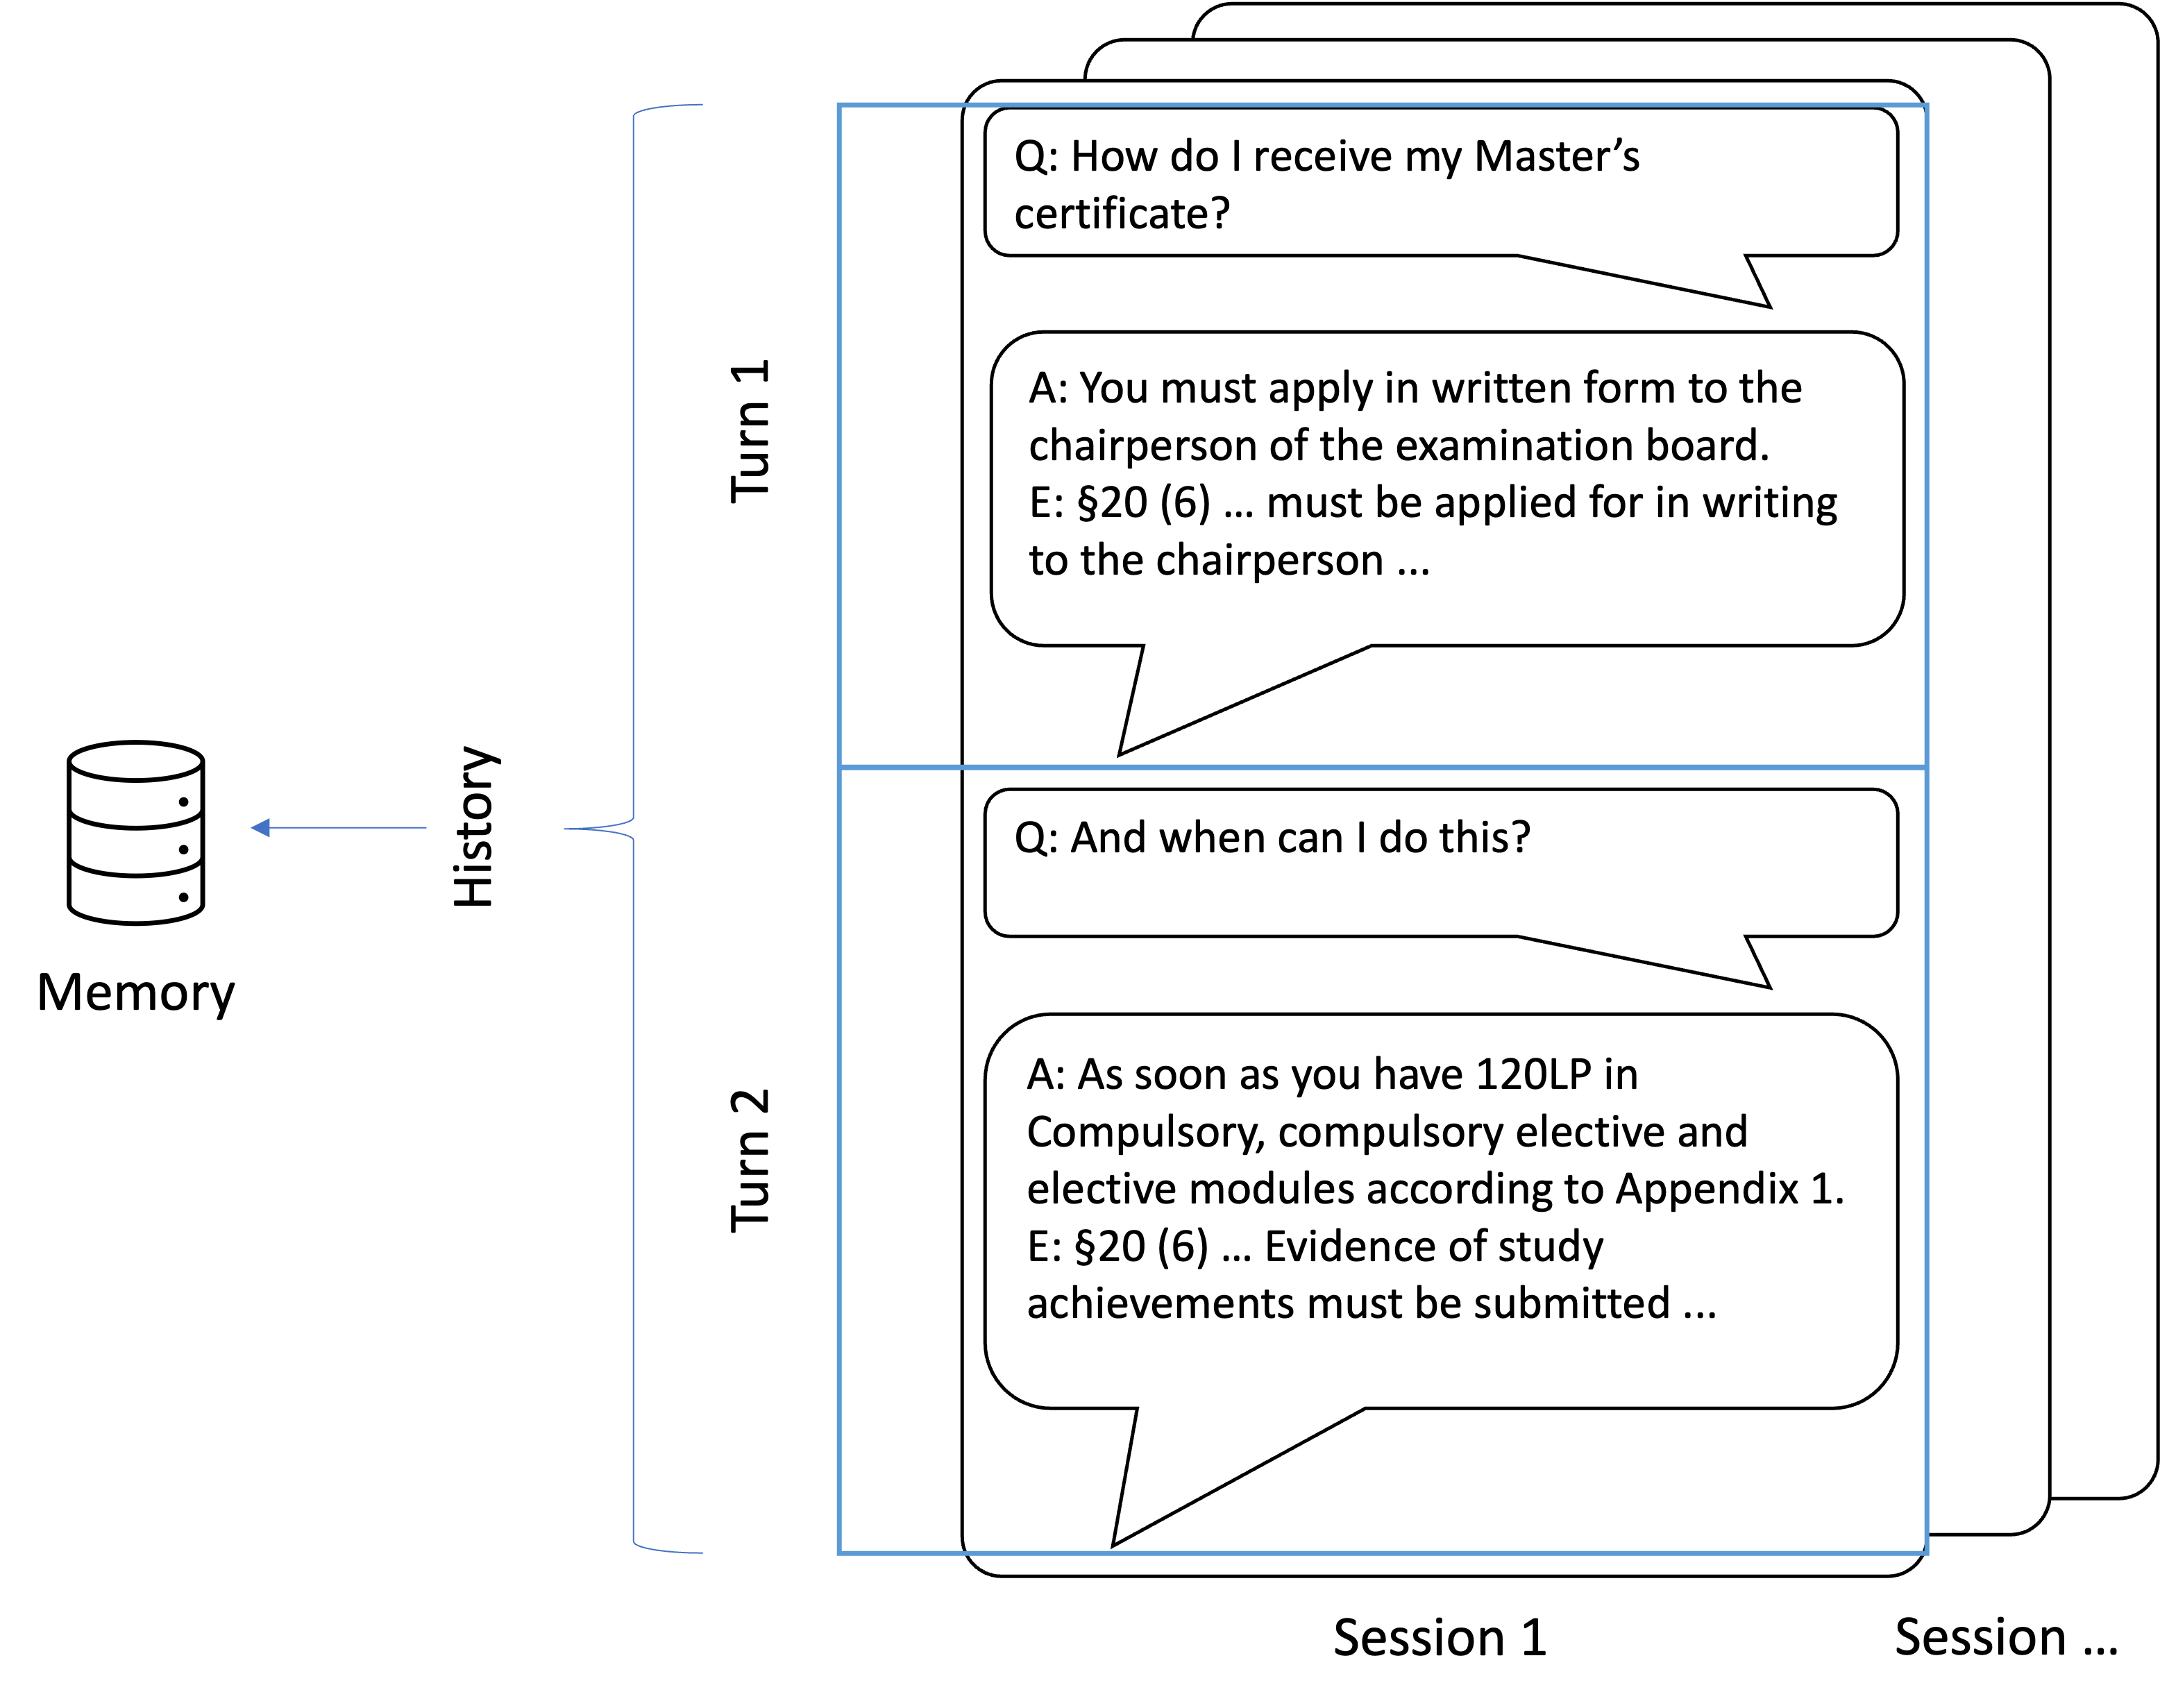
\includegraphics[width=\textwidth]{Grafiken/Conversation_Explain.png}
        \captionsetup{font={tiny}} % This line changes the caption font size
        \caption{Concepts of a Conversation in regards to a CIS}
      \end{figure}
      \vfill
    \end{column}
    
    \begin{column}{.4\textwidth}
      \vfill
      Important Concepts:
      \begin{itemize}
        \item Turn - A user question and system answer.
        \item History - Previous turns in a session.
        \item Session - A complete conversation.
        \item Memory - System's knowledge of the conversation(s).
      \end{itemize}
      \vfill
    \end{column}
  \end{columns}

\end{frame}

\section[Problem Statement]{Problem Statement}

\begin{frame}{QA-System}
  \begin{enumerate}
    \item Utilize \textbf{documents} as the primary \textbf{knowledge source}.
    \item Enable the QA-System to handle a \textbf{variety of answer types}, including: \textbf{extractive}, \textbf{abstractive}, and \textbf{boolean}.
    \item \textbf{Provide references} to document snippets \textbf{as evidence to answers}.
    \item Ensure the pipeline's generalizability by using \textbf{open-domain methods}, allowing it to adapt to new domains or knowledge sources with \textbf{minimal or no supervision} and \textbf{small datasets}.
    \item Design the pipeline to be \textbf{feasible without the need for datacenter-grade hardware resources}, making it accessible for development on standard research hardware.
  \end{enumerate}
\end{frame}
  
\begin{frame}{QA-System (cont.) and Conversationality}
  \begin{enumerate}
    \setcounter{enumi}{5}
    \item \textbf{Prioritize accuracy as the primary objective}, as constraining memory consumption is indirectly covered in point (5). \textbf{Latency is not a primary concern}, as the system is not intended for real-time use and will not be optimized for that in this thesis.
  \end{enumerate}
  
  Conversationality:
  \begin{enumerate}
    \item Enable the ConvQA-System to \textbf{handle} the following follow-up \textbf{question types: drilling-down, clarification, topic shift} and \textbf{comparison}.
    \item Be able to take Initiative in the form of \textbf{clarifying questions}.
    \item The \textbf{memory} will be \textbf{limited to a session} and not multi-session.
  \end{enumerate}
\end{frame}

\begin{frame}{Problem Definition}

  \begin{figure}
    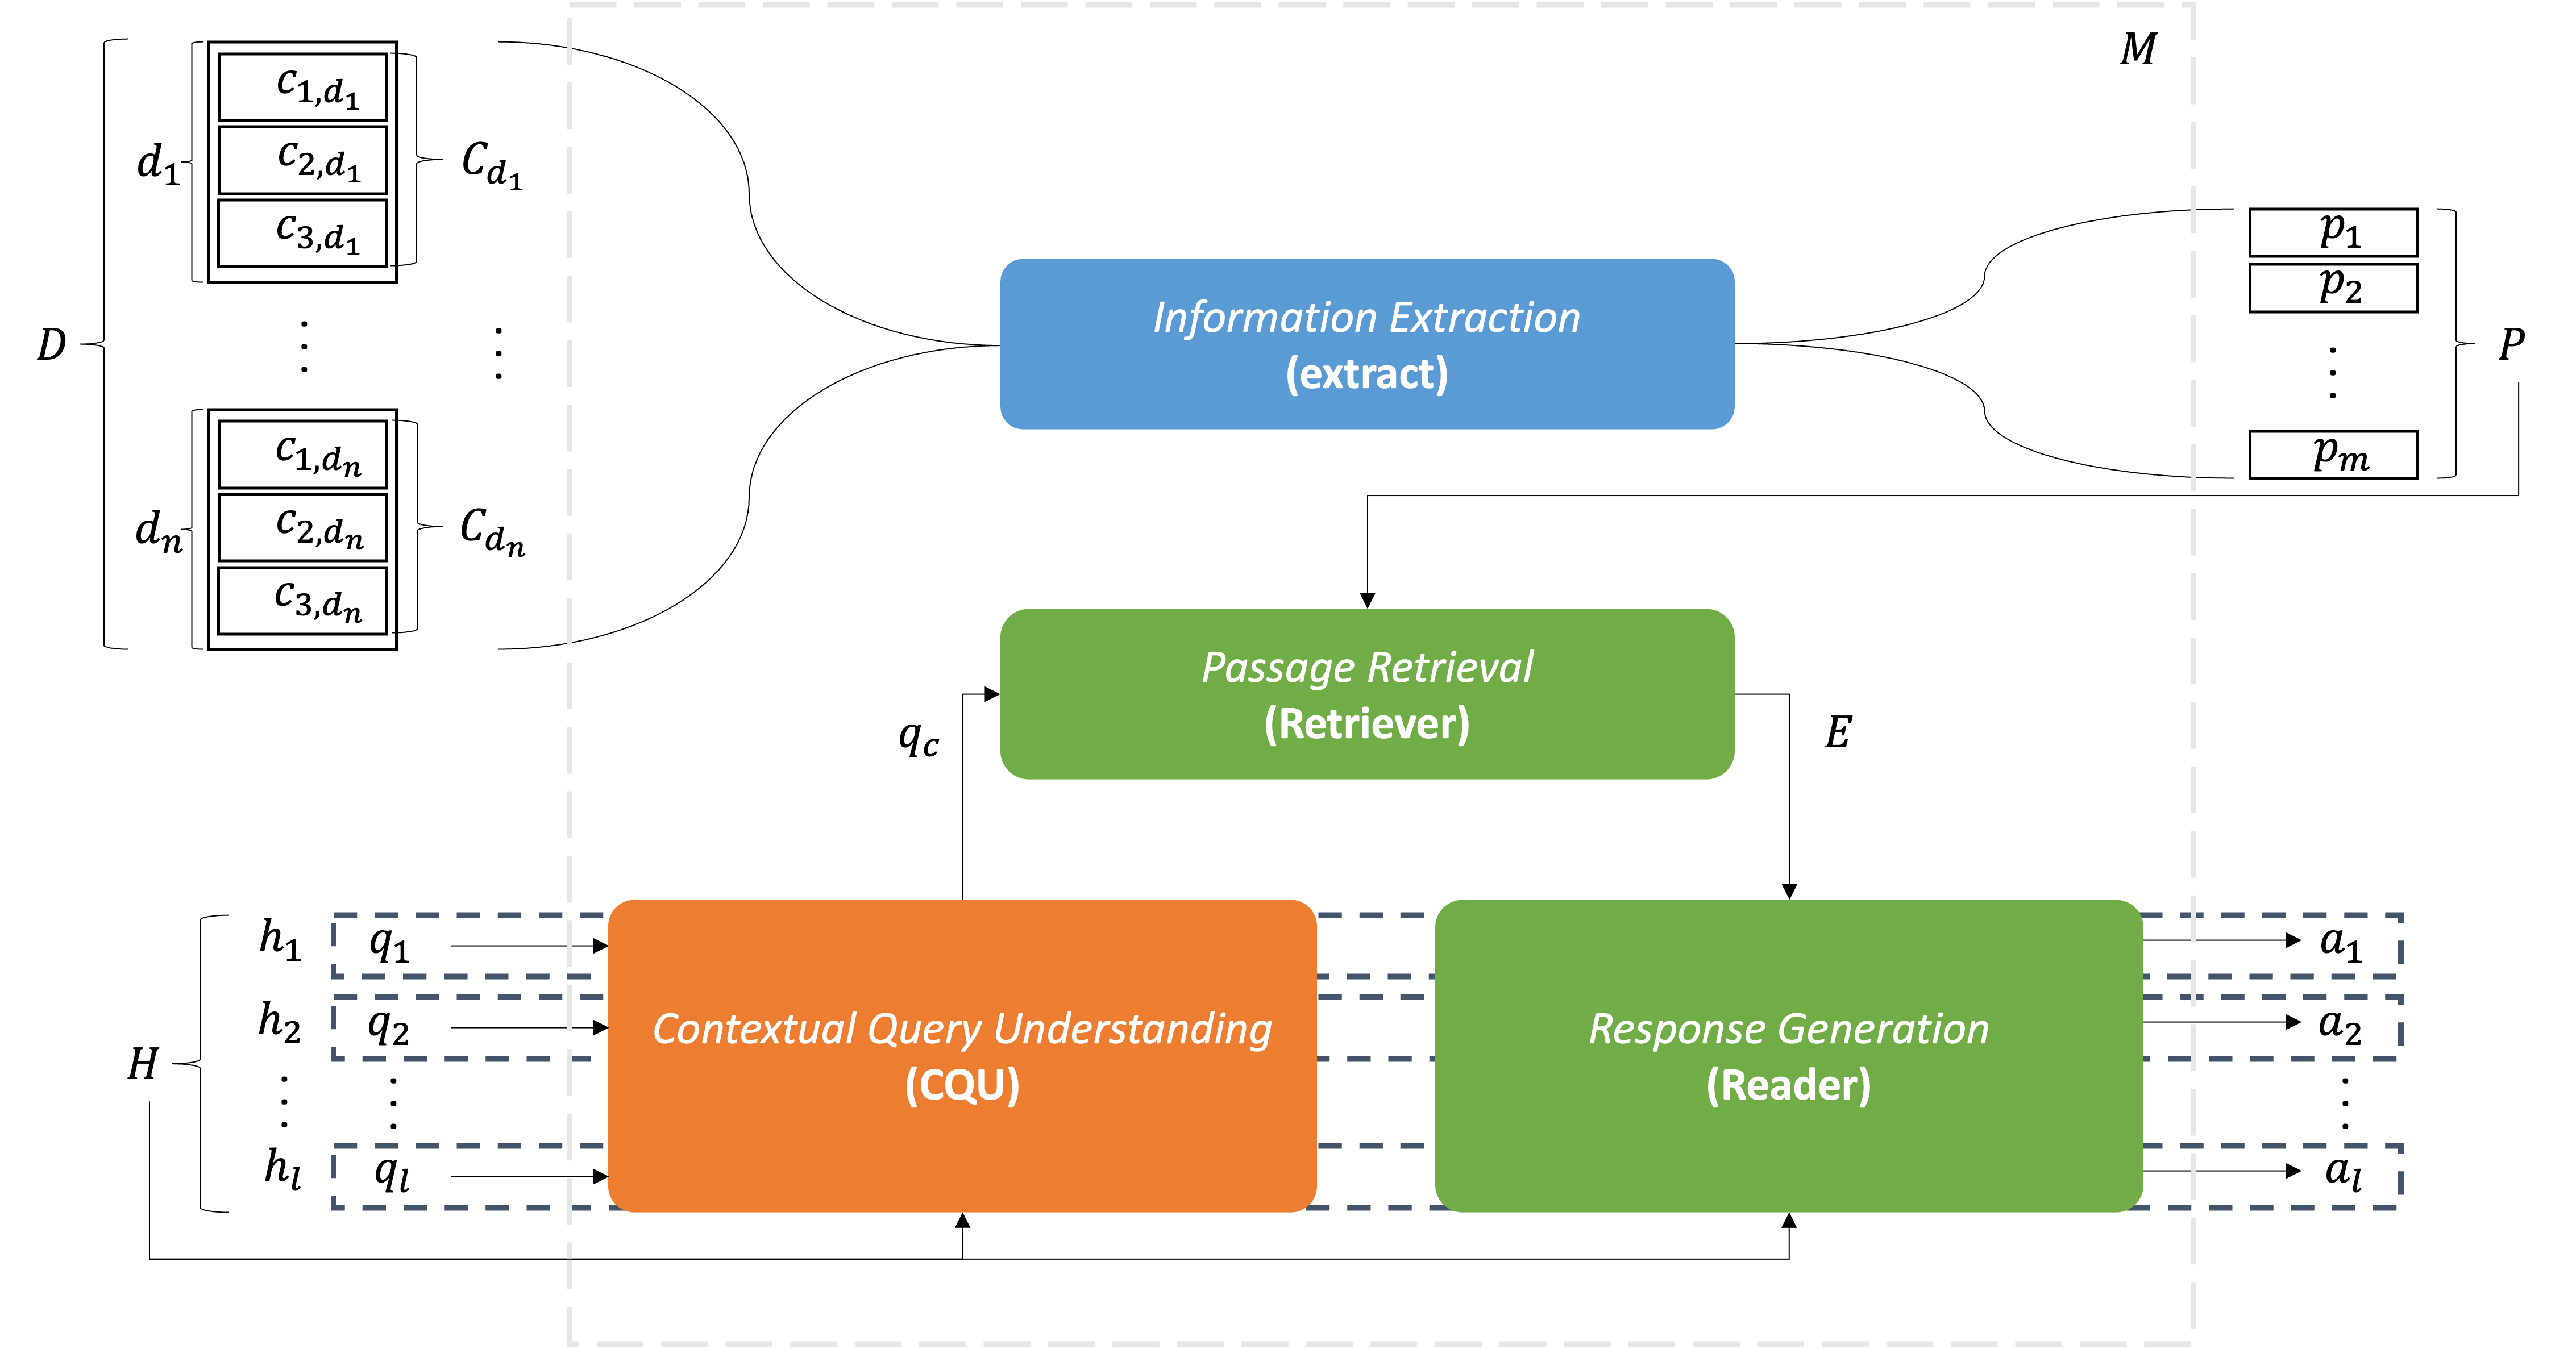
\includegraphics[width=\textwidth]{Grafiken/conrag_konzeptionell.png}
    \captionsetup{font={tiny}} % This line changes the caption font size
    \caption{Abstract System Architecture $\mathbf{M}$}
  \end{figure}
  
\end{frame}

\begin{frame}{Definition Intent}
  
  \begin{definition}
    \textbf{(Intent)} Given two elements, which either can be questions, answers or passages, there exists an operation Intent $\mathcal{I}(x, y)$. This operation returns a value between 0 and 1, which indicates the overlap of the two intents of $x$ and $y$, $\mathcal{I}(x, y) = [0,1]$.
    \label{def:intent}
  \end{definition}

  \bigskip
  \textbf{Example:}
  \begin{flushleft}
    Question: When was Barack Obama born?
  \end{flushleft}
  \begin{flushleft}
    Answer 1: 4. August 1961

    Answer 2: Barack Obama was the 44th president of the USA.
    
    Answer 3: Either 04.08.1961 or 05.09.1962 I'm not sure. 
  \end{flushleft}

\end{frame}

\section[ConRAG]{Conversationl RAG}

\begin{frame}{Conversational RAG}

  \vfill
  \begin{figure}
    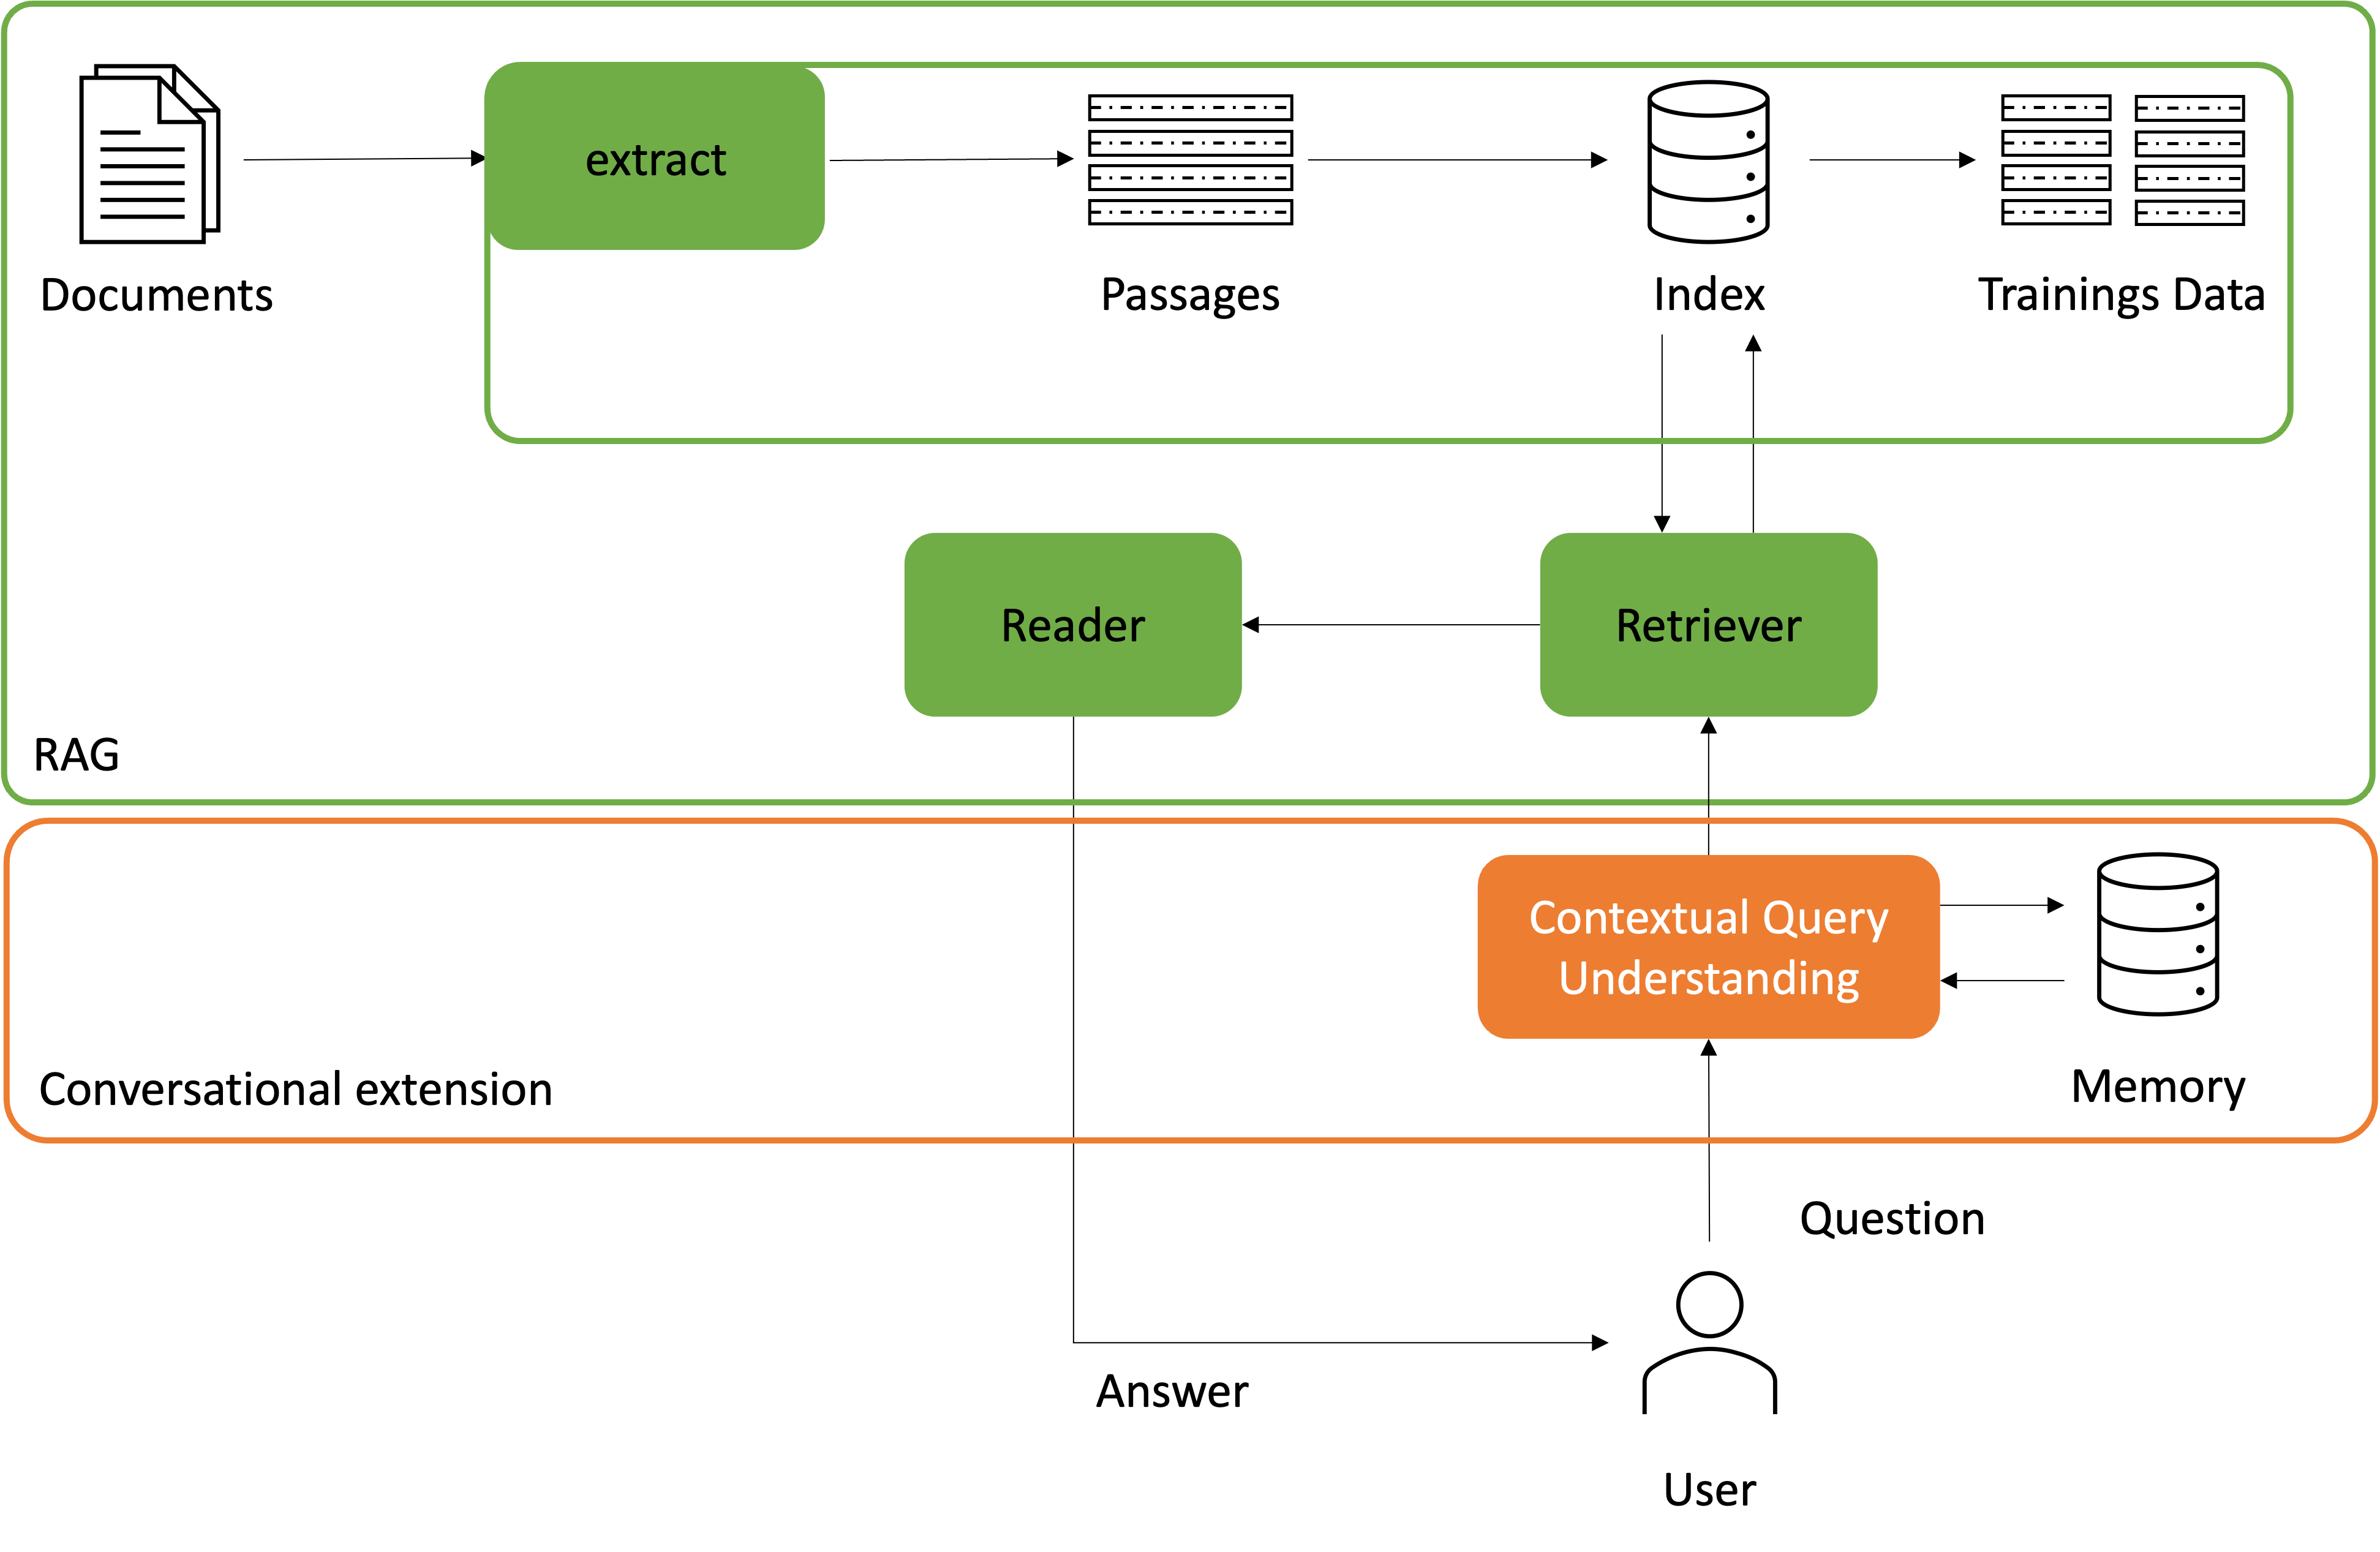
\includegraphics[width=0.9\textwidth]{Grafiken/System_Architecture.png}
    \captionsetup{font={tiny}} % This line changes the caption font size
    \caption{Overview of the Conversational-RAG System Architecture}
  \end{figure}
  \vfill

\end{frame}

\subsection*{Extract}
\begin{frame}{Extract}

  \begin{block}{Definition}
    \textbf{(Extraction)} Given a set of documents $D$, extract the textual content $C_d$ of each document $d \in D$ and create a knowledge source $P$ based on $C_d$ of every document $d \in D$. 
  \end{block}

  \begin{columns}[T] % align columns
    \begin{column}{.5\textwidth}
      {\color{unirot}Operations}
      \begin{itemize}
        \item Information Extraction
        \begin{itemize}
          \item Structured Extraction
          \item Unstructured Extraction
        \end{itemize}
        \item Passage Extraction 
        \begin{itemize}
          \item Paragraphs
          \item Snippets
          \item Sliding Window
        \end{itemize}
      \end{itemize}
    \end{column}
    
    \begin{column}{.5\textwidth}
      {\color{unirot}Synthetic Data}
      \begin{itemize}
        \item Questions given Context
        \item Question-Context-Answer Triples
        \item Conversational Question-Context-Answer Histories
      \end{itemize}
    \end{column}
  \end{columns}
\end{frame}

\subsection*{Retriever}
\begin{frame}{Retriever - Overview}
  \vfill

  \begin{block}{Definition}
    \textbf{(Retriever)} Given a contextualized question $q_c$ and a knowledge source $P$, retrieve the most relevant passages $p$ from $P$ and combine them in an evidence set $E$.
  \end{block}

  \begin{figure}
    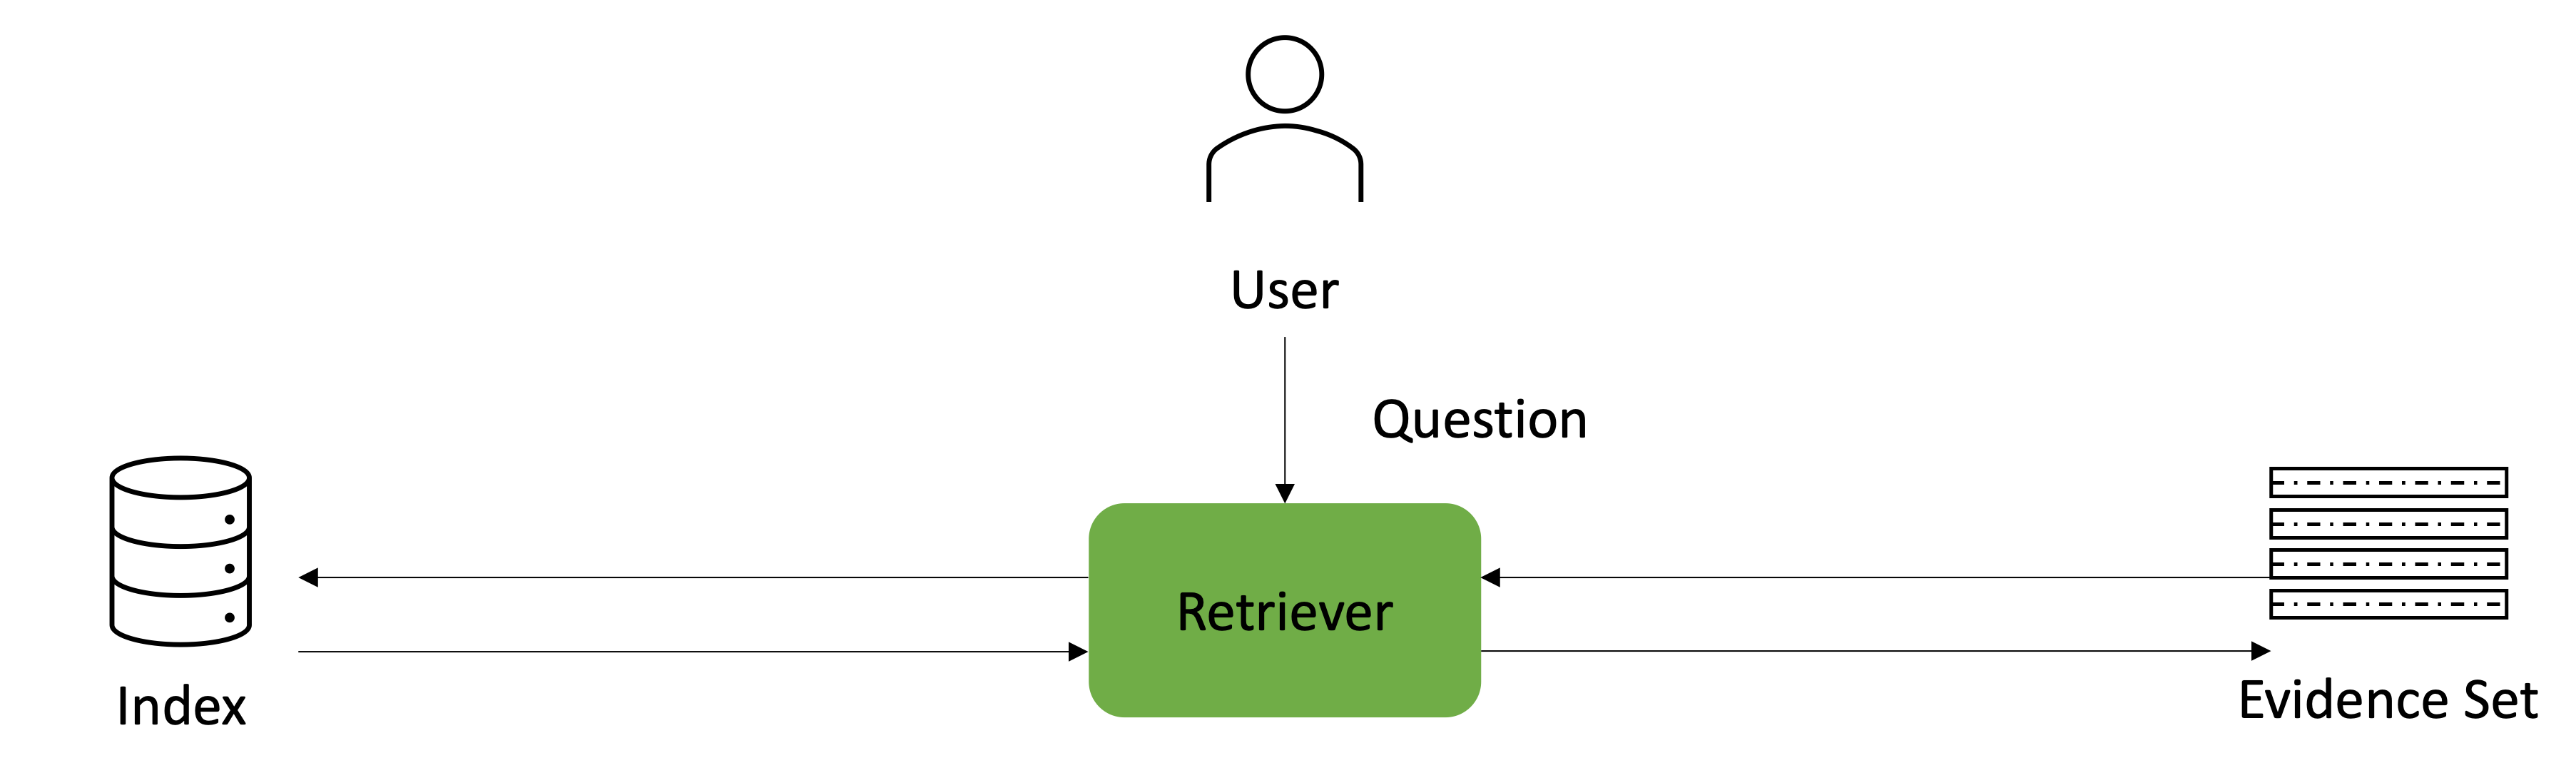
\includegraphics[width=\textwidth]{Grafiken/Retriever_Fields_of_Improvement.png}
    \captionsetup{font={tiny}} % This line changes the caption font size
    \caption{Retriever Relations}
  \end{figure}
\end{frame}

\begin{frame}{Retriever - Index}
  \begin{figure}
    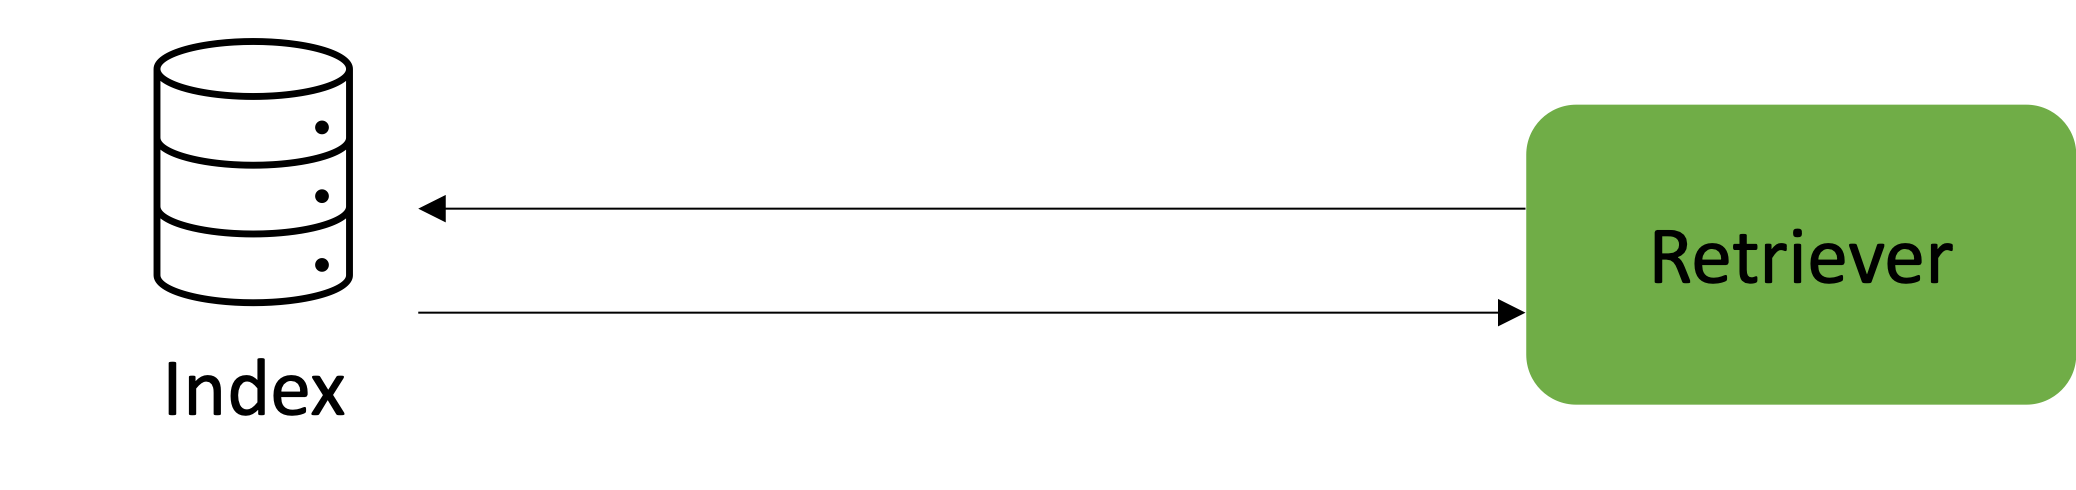
\includegraphics[width=0.4\textwidth]{Grafiken/Retriever_Index.png}
  \end{figure}

  \begin{block}{Fine-Tuning}
    \begin{columns}
      \begin{column}{.55\textwidth}
        \begin{figure}
          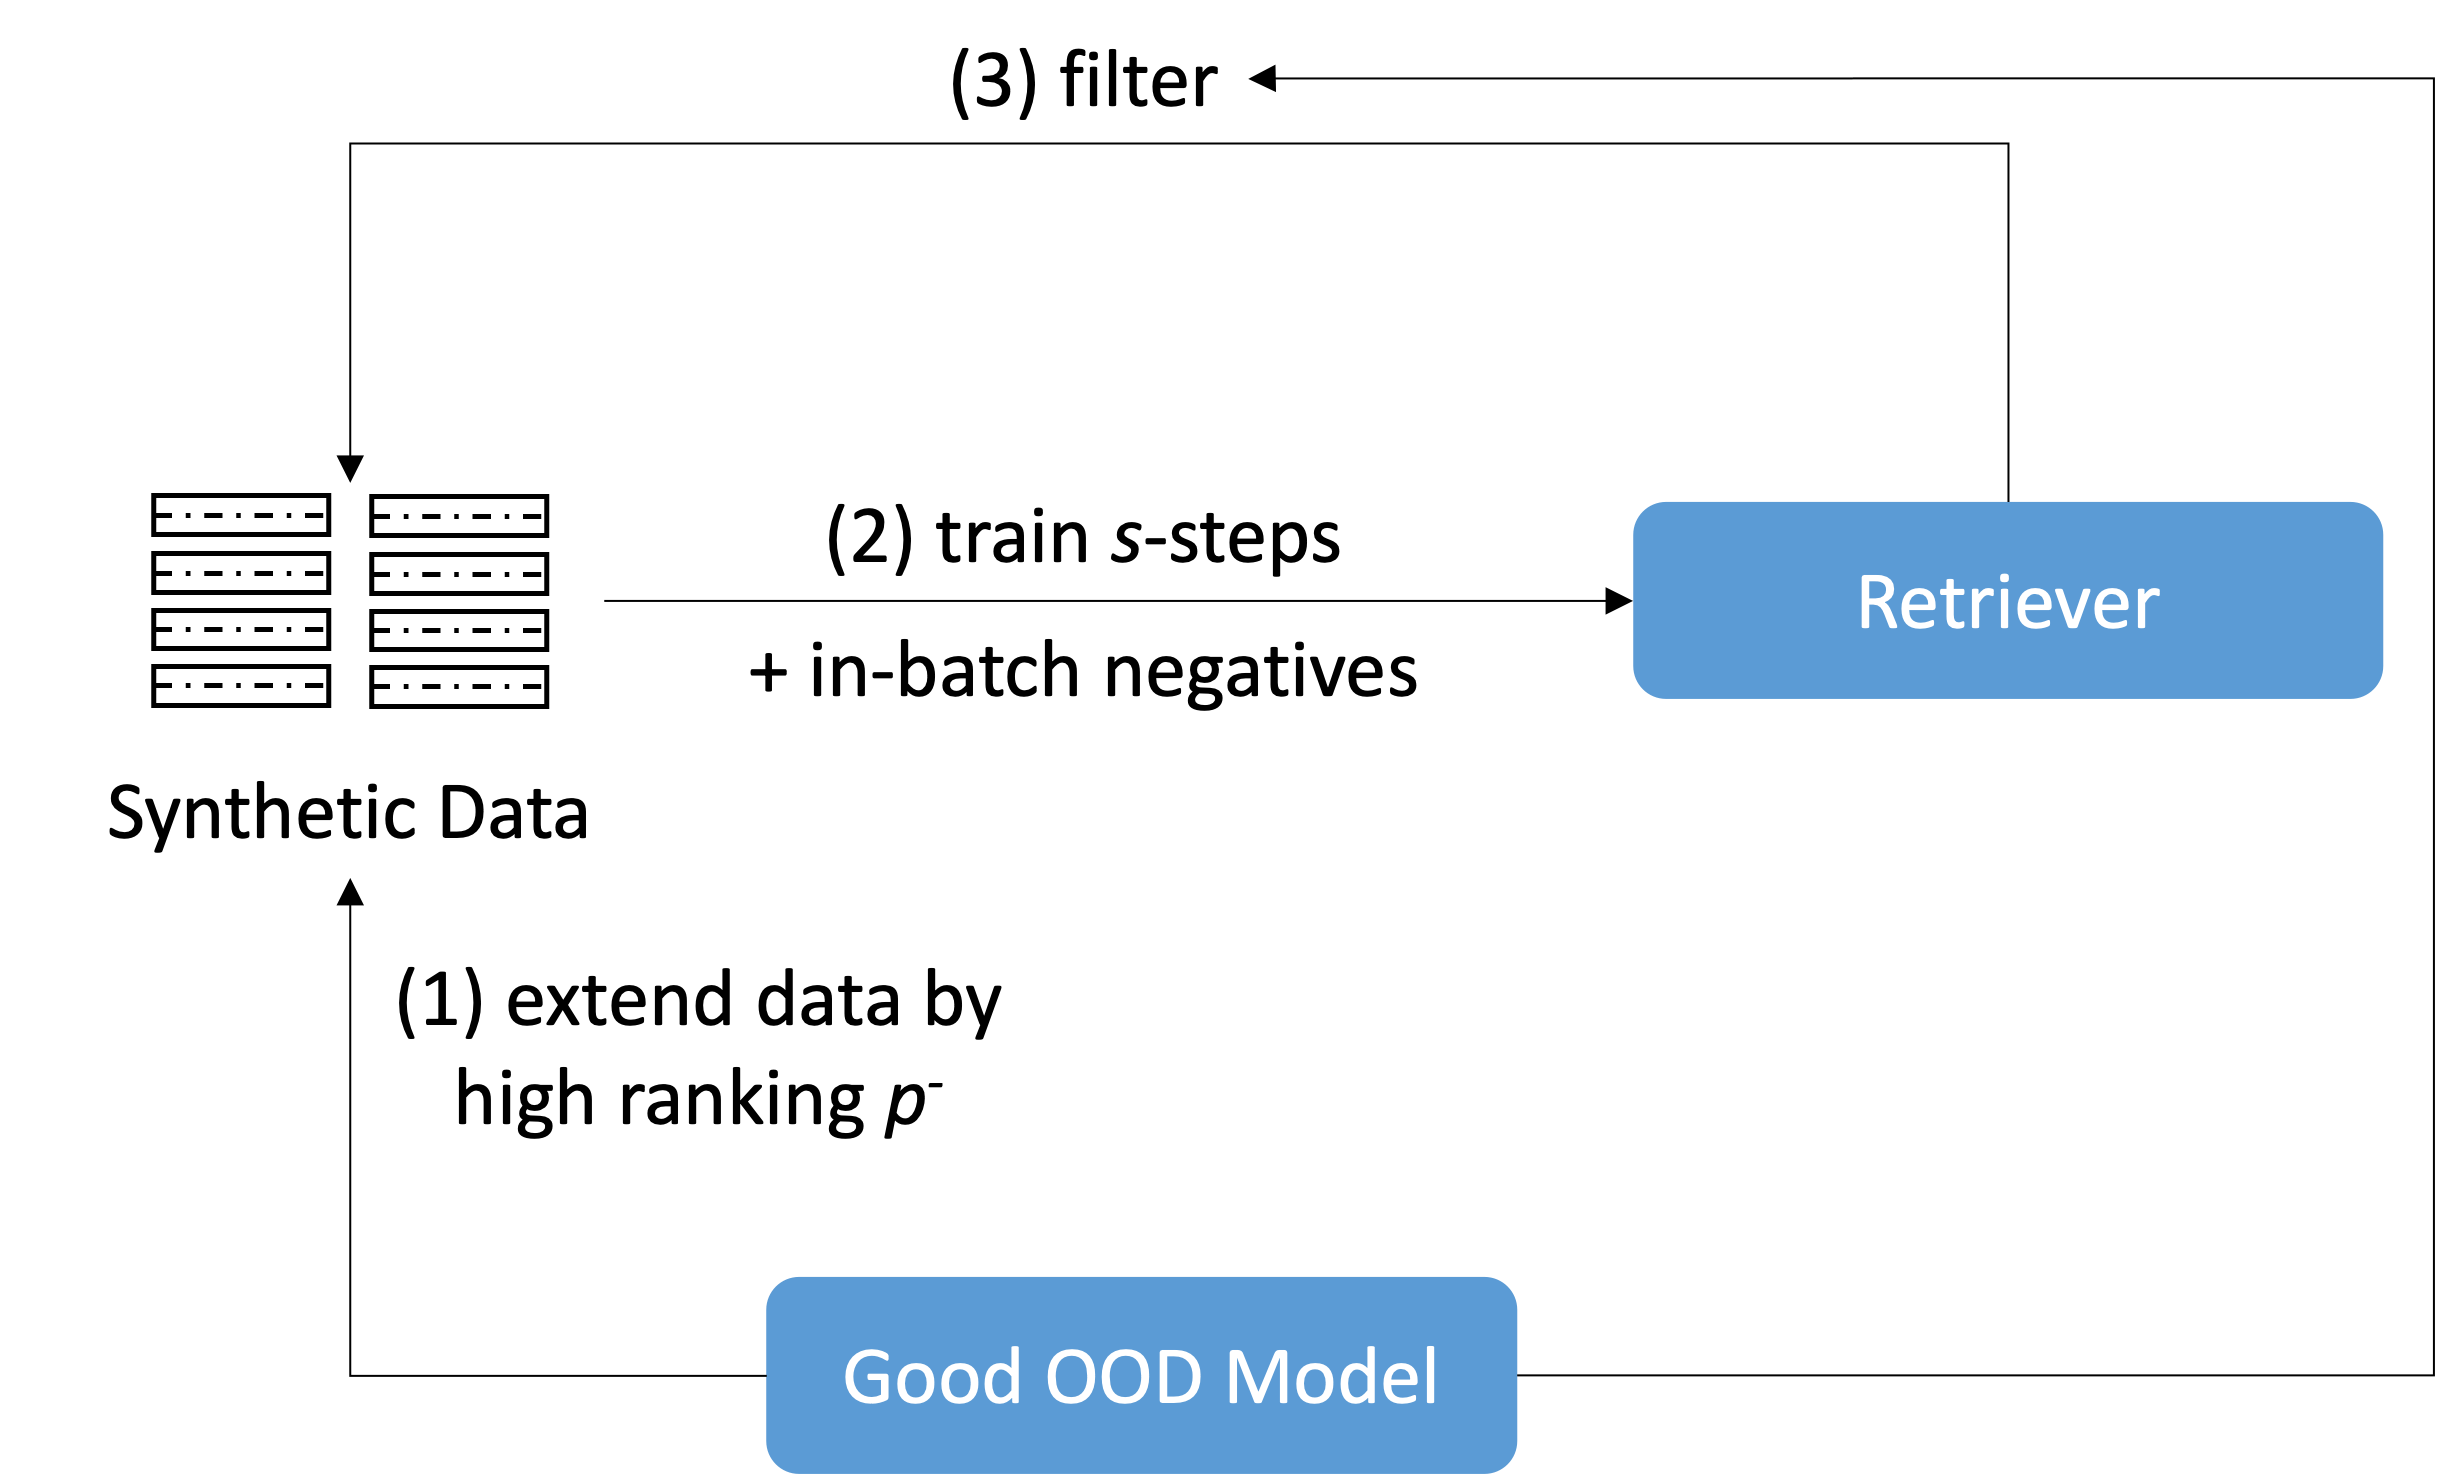
\includegraphics[width=0.9\textwidth]{Grafiken/Training.png}
          \captionsetup{font={tiny}} % This line changes the caption font size
          \caption{Fine-Tuning of the Retriever}
        \end{figure}
      \end{column}

      \begin{column}{.45\textwidth}
        \begin{itemize}
          \item Use synthetic Q-A pairs
          \item Adapt Retriever to Passage language and format 
          \item Filter out incorrect synthetic pairs
        \end{itemize}
      \end{column}
    \end{columns}
  \end{block}
  \vfill
\end{frame}

\begin{frame}{Retriever - Metadata}
  \begin{figure}
    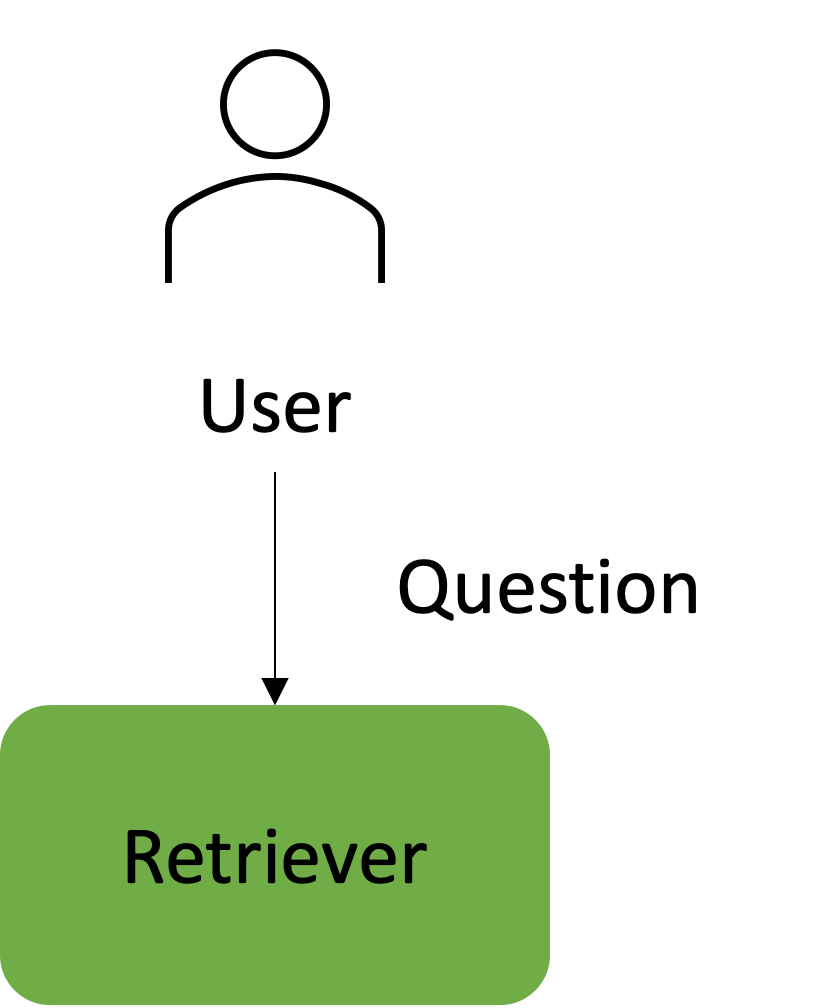
\includegraphics[width=0.15\textwidth]{Grafiken/User_Retriever.png}
  \end{figure}

  \begin{block}{Metadata Filtering}


\begin{columns}
  \begin{column}{.4\textwidth}
    \vfill
    \small
    \scalebox{0.7}{$
        m_{\text{Ret}}(p|q_c) =
        \begin{cases}
                p \in E_m, & \bigcap\limits_{i=p_1}^{\substack{E_{q_c}}} M_{i} \subset M_p \\
                p \notin E_m, & \bigcap\limits_{i=p_1}^{\substack{E_{q_c}}} M_{i} \not\subset M_p
        \end{cases}
    $}
    \vfill
    \normalsize
  \end{column}
  \begin{column}{.5\textwidth}
    \textbf{Index Types:}
    \begin{itemize}
      \item Metadata Passage Integration
      \item Separate Metadata Index
      \item Hierarchical Index
    \end{itemize}
  \end{column}
\end{columns}


  \end{block}
\end{frame}

\begin{frame}{Retriever - Evidence Set}
  \begin{figure}
    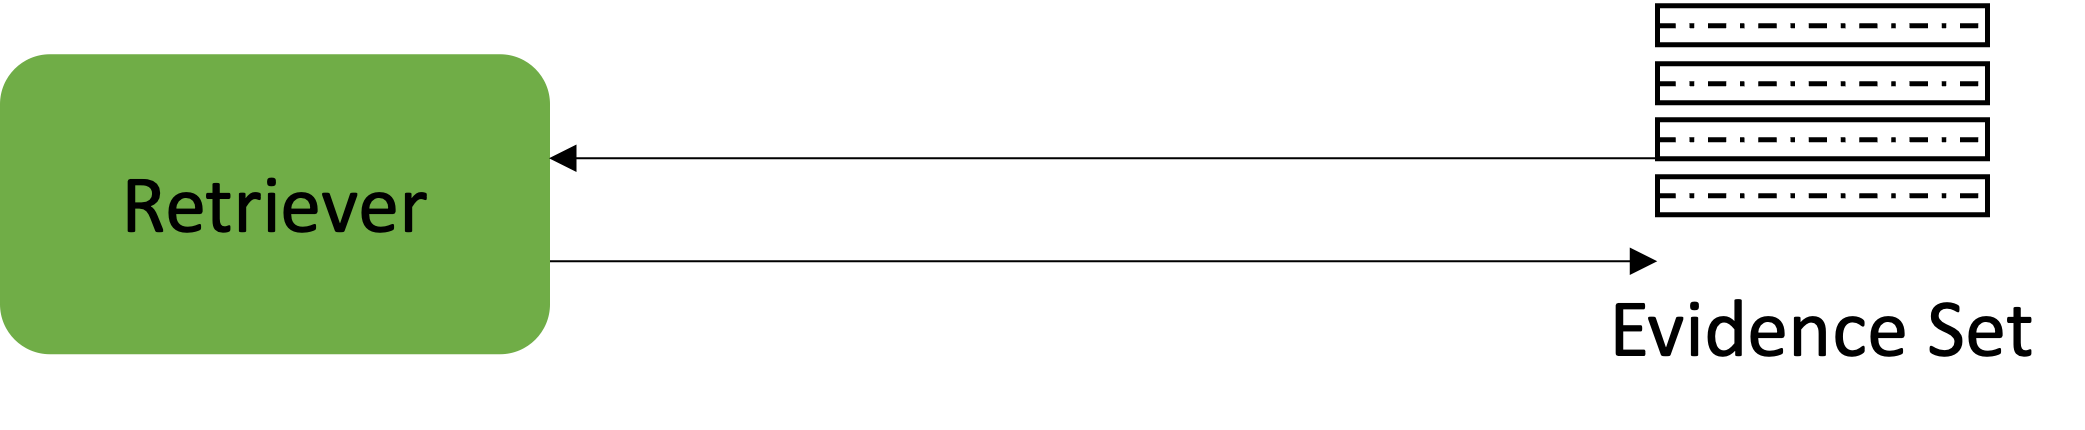
\includegraphics[width=0.4\textwidth]{Grafiken/Retriever_Passages.png}
  \end{figure}

  \begin{block}
    {Mixture-of-Experts}
    \textbf{Approaches:}
    \begin{itemize}
      \item Re-Ranking
      \item Ensemble
    \end{itemize} 
  \end{block}
\end{frame}

\subsection*{Reader}

\begin{frame}
  \frametitle{Reader - Challenges}

  \begin{block}{Definition}
    \textbf{(Reader)} Given a history $H$, a new question $q_{i+1}$ and a set of passages $E$, generate an answer $a$ to $q_{i+1}$ based on $E$, so that $\mathcal{I}(q_{i+1},a) = 1$.
  \end{block}

  \textbf{Challenges:}

  \begin{enumerate}
    \item Generate an answer $a$ based on $E_{q_c}$ that satisfies $\mathcal{I}(q_c, a) = 1$.
    \item Identify the case for $E_{q_c}$ and determine $\hat{E}_{q_c} \subset E_{q_c}, \quad \mathcal{I}(q_c, \hat{E}_{q_c}) = 1$.
    \item Identify ambiguous questions $q_{i}$ and determine a clarification question $a_{i}$ for the next turn $i+1$.
    \item Ensure chatlike behavior, including contextual understanding and human-like conversation.
  \end{enumerate}

\end{frame}

\begin{frame}{Reader - Solutions}

  \textbf{Solutions:}

  \begin{enumerate}
    \item Train the model with a dataset of varied question-context-answer triples where context is $\hat{E}_{q_c}$ and the question type varies.
    \item Implement a passage identification mechanism in the Reader to overcome Transformer context window limitations and nonperfect evidence sets. Solutions:
      \begin{itemize}
          \item Re-Ranker: Re-rank $E_{q_c}$ before Reader processing.
          \item Compression: Extract most relevant information from passage $p \in E_{q_c}$.
          \item Multi-Retrieval: Perform multiple retrievals until evidence set $E_{q_c}$ is satisfactory.
          \item Trained Reader: Train Reader on a dataset where $E_{q_c} \not= \hat{E}_{q_c}$.
          \item Parametric Knowledge: Train Reader's Transformer on knowledge source $P$.
      \end{itemize}
  \end{enumerate}
  
\end{frame}

\begin{frame}{Reader - Solutions (cont.)}

  \textbf{Solutions (continued):}

  \begin{enumerate}
    \setcounter{enumi}{2}
    \item Train on a dataset with question-context-answer-ambiguity quadruples to learn to identify and resolve ambiguous questions.
    \item Fine-tune a Transformer model for human-like conversation using a human conversation history dataset $H$.
  \end{enumerate}
  
\end{frame}


\subsection*{Contextual Querry Understanding}

\begin{frame}{Contextual Query Understanding}

  \begin{block}{Definition}
    \textbf{(CQU)} Given a history $H$ and a new question $q_{i+1}$, generate a contextualized question $q_c$ based on $H$, such that $\mathcal{I}(q_c,q_{i+1}) = 1$. 
  \end{block}

  \begin{equation*}
    CQU(h_{i-k:i}, q_{i+1}) := q_c \mid \mathcal{I}(q_c, q_{i+1}) = 1
  \end{equation*}

  \bigskip

  \begin{enumerate}
    \item \textbf{K-many:} Consideration of the last $k$ turns.
    \item \textbf{All:} Utilization of the entire history, $k = i - 1$.
    \item \textbf{Memory:} Inclusion of not only the current history but also previous Sessions by this user.
  \end{enumerate} 
\end{frame}

\section[Implementation]{Implementation}

\subsection{Dataset}


\begin{frame}{Dataset}
  \begin{columns}
    \begin{column}{.5\textwidth}
      \begin{figure}
        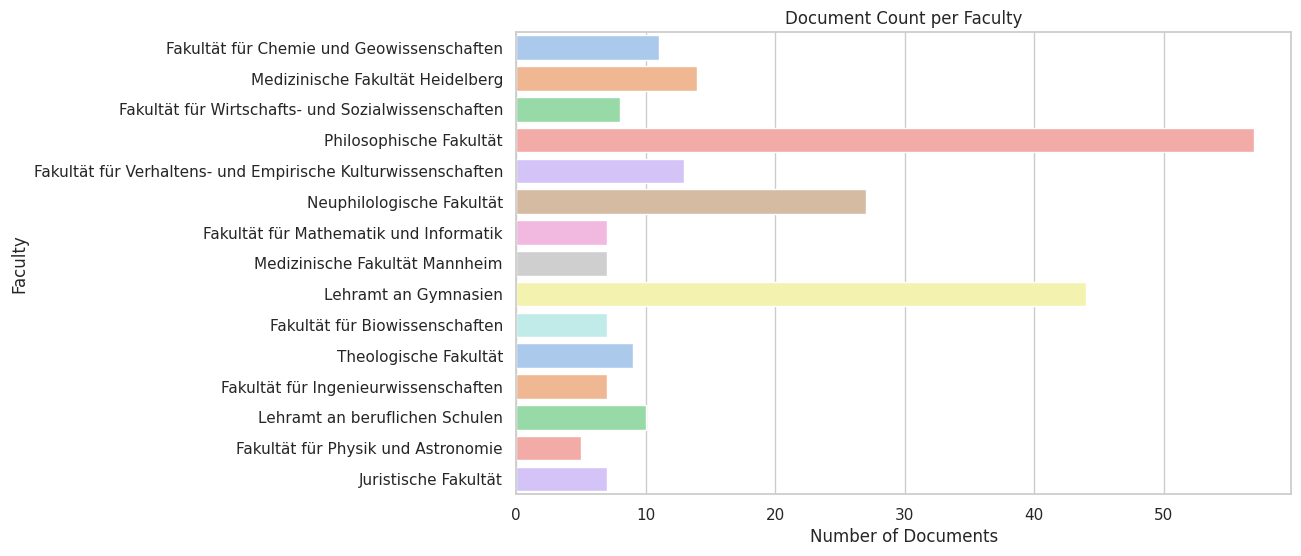
\includegraphics[width=0.9\textwidth]{Grafiken/PO_german_Document Count per Faculty.png}
        \captionsetup{font={tiny}} % This line changes the caption font size
        \caption{Documents per Faculty - German ERs}
      \end{figure}
      \begin{figure}
        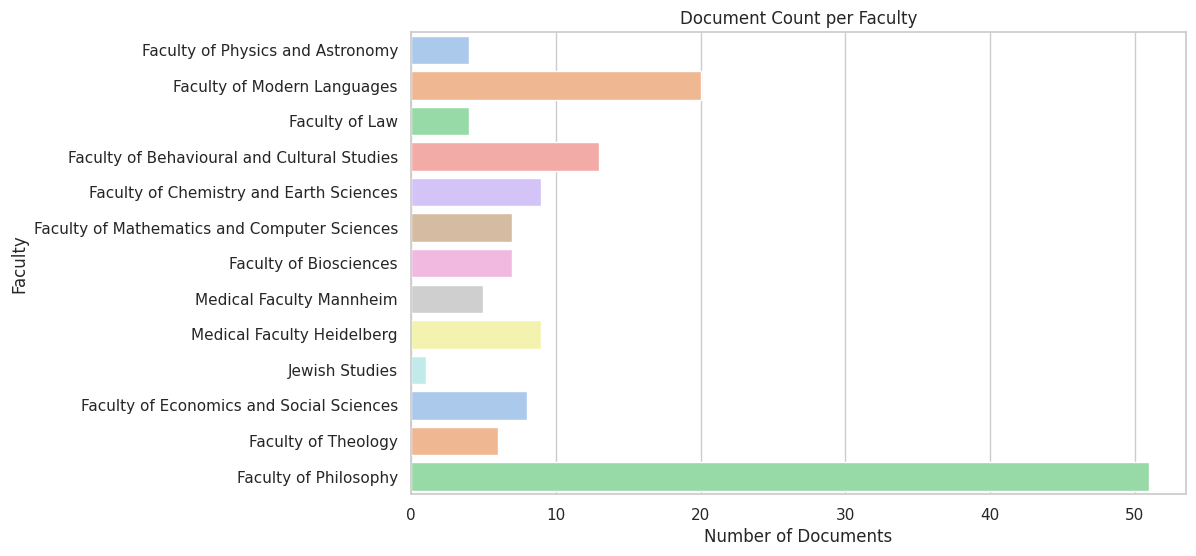
\includegraphics[width=0.9\textwidth]{Grafiken/PO_english_Document Count per Faculty.png}
        \captionsetup{font={tiny}} % This line changes the caption font size
        \caption{Documents per Faculty - English ERs}
      \end{figure}
    \end{column}
    \begin{column}{.5\textwidth}
      \begin{figure}
        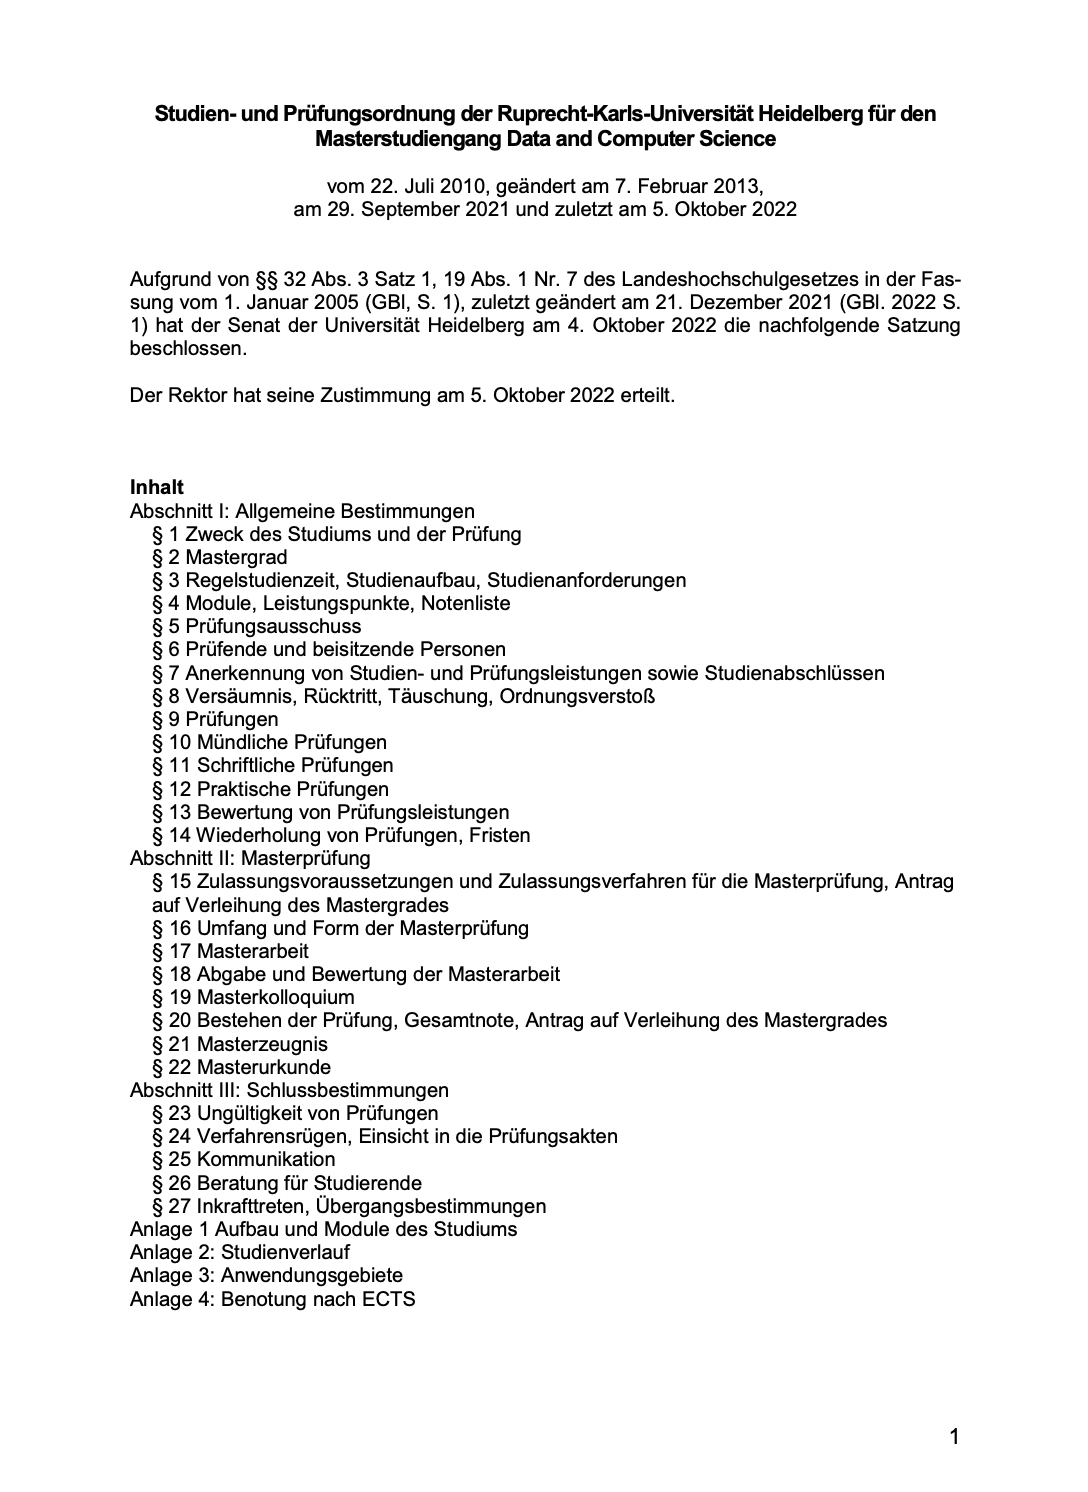
\includegraphics[width=0.9\textwidth]{Grafiken/DnC_PO.png}
        \captionsetup{font={tiny}} % This line changes the caption font size
        \caption{Example PDF of the Dataset}
      \end{figure}
    \end{column}
  \end{columns}
\end{frame}

\subsection{Extract}

\begin{frame}
  \frametitle{Extract Statistics}

  \begin{figure}
    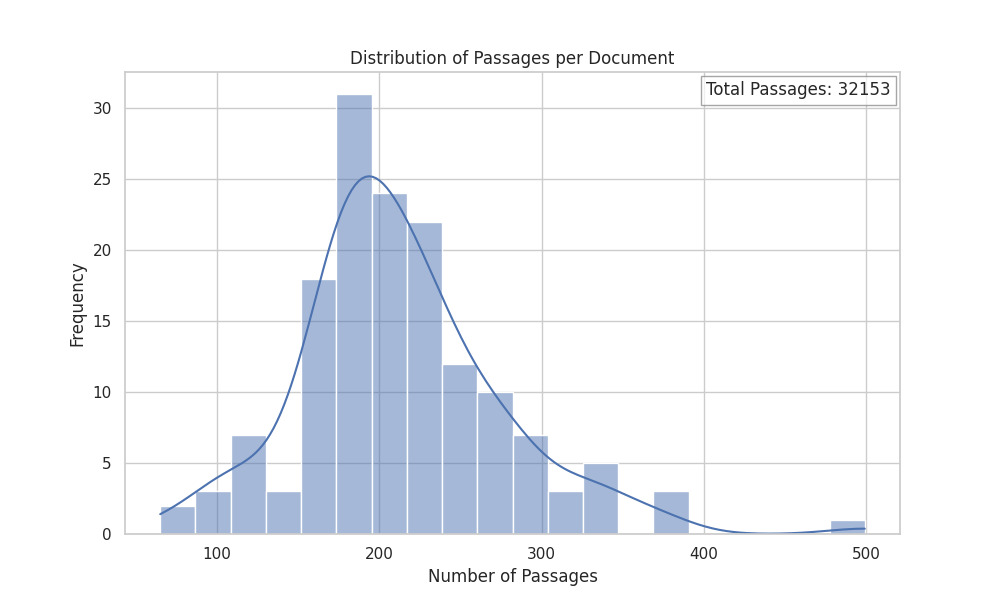
\includegraphics[width=0.5\textwidth]{Grafiken/IndexEnglish_Passages_Distribution.png}
    \captionsetup{font={tiny}}
    \caption{Passages per Document of the English Dataset}
  \end{figure}

  \begin{figure}
    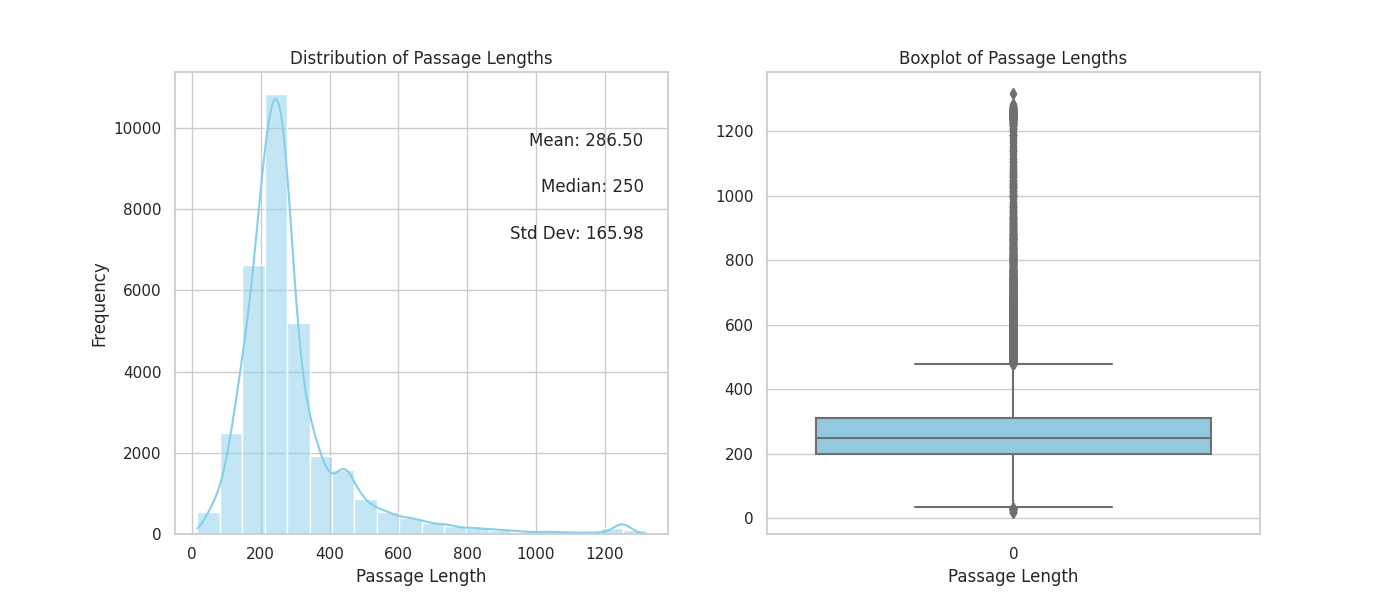
\includegraphics[width=0.5\textwidth]{Grafiken/IndexEnglish_Passage_Length_Statistics.png}
    \captionsetup{font={tiny}}
    \caption{Passage Length Distribution of the English Dataset} 
  \end{figure}

\end{frame}

\subsection{Models}

\begin{frame}{Used Models}

  \begin{center}
    {\color{unirot}Retriever}
  
    \begin{table}[]
      \scriptsize
      \renewcommand{\arraystretch}{1.5} % Add more vertical spacing to the table
      \begin{tabular}{|l|l|}
      \hline
      \textbf{Model} & \textbf{Notes} \\ \hline
      \textit{BM25}\footnotemark[1] & $k_1$ = 1.5, b = 0.75, c = 0.25 \\ \hline
      % \textit{BM25 + CE} & English: \emph{ms-marco-MiniLM-L-6-v2}\footnotemark[2], German: \emph{ms-marco-MiniLM-L-6-en-de-v1}\footnotemark[3] \\ \hline
      \textit{BM25 + CE} & \begin{tabular}{@{}l@{}}
                            English: \emph{ms-marco-MiniLM-L-6-v2}\footnotemark[2] \\
                            German: \emph{ms-marco-MiniLM-L-6-en-de-v1}\footnotemark[3]
                          \end{tabular} \\ \hline
      \textit{Large DPR} & English/German: \emph{text-embedding-ada-002}\footnotemark[4] \\ \hline
      \end{tabular}
      \captionsetup{font={tiny}}
      \caption{Used Retriever Models}
      \label{tab:retriever-models}
    \end{table}
  \end{center}

  \begin{center}
    {\color{unirot}Reader}
    \begin{table}[]
      \scriptsize
      \renewcommand{\arraystretch}{1.5} % Add more vertical spacing to the table
      \begin{tabular}{|l|l|}
      \hline
      \textbf{Model} & \textbf{Parameters} \\ \hline
      \textit{GPT-3.5-turbo}\footnotemark[5] & Approx. 175B \\ \hline
      \textit{Llama2-7B-chat-GPTQ}\footnotemark[6] & 7B \\ \hline
      \textit{leo-hessianai-7B-chat-GPTQ}\footnotemark[7] & 7B \\ \hline
      \end{tabular}
      \captionsetup{font={tiny}}
      \caption{Used Reader Models}
      \label{tab:reader-models}
    \end{table}
  \end{center}

\end{frame}


% \begin{frame}{Used Models}
%   \begin{columns}[T] % Added [T] option for top alignment
%     \begin{column}{.5\textwidth}
%       \textbf{Retriever}
%       \begin{itemize}
%         \item BM25\footnotemark[1]
%           \begin{itemize}
%             \item k\_1 = 1.5, b = 0.75, c = 0.25
%           \end{itemize}
%         \item BM25 + CE
%           \begin{itemize}
%             \item English: \emph{ms-marco-MiniLM-L-6-v2}\footnotemark[2]
%             \item German: \emph{ms-marco-MiniLM-L-6-en-de-v1}\footnotemark[3]
%           \end{itemize}
%         \item Large DPR
%           \begin{itemize}
%             \item \emph{text-embedding-ada-002}\footnotemark[4]
%           \end{itemize}
%       \end{itemize}
%     \end{column}
%     \begin{column}{.5\textwidth}
%       \textbf{Reader}
%       \begin{itemize}
%         \item \emph{gpt-3.5-turbo} (approx. 175B)\footnotemark[5]
%         \item \emph{Llama2-7B-Chat-GPTQ}\footnotemark[6]
%         \item \emph{leo-hessianai-7B-chat-GPTQ}\footnotemark[7]
%       \end{itemize}
%     \end{column}
%   \end{columns}
% \end{frame}

\section[Experiments]{Experiments}

\subsection*{Evaluation Methods}

\begin{frame}{Evaluation of RAG}
    
  \captionsetup{font={tiny}}
  \begin{figure}
    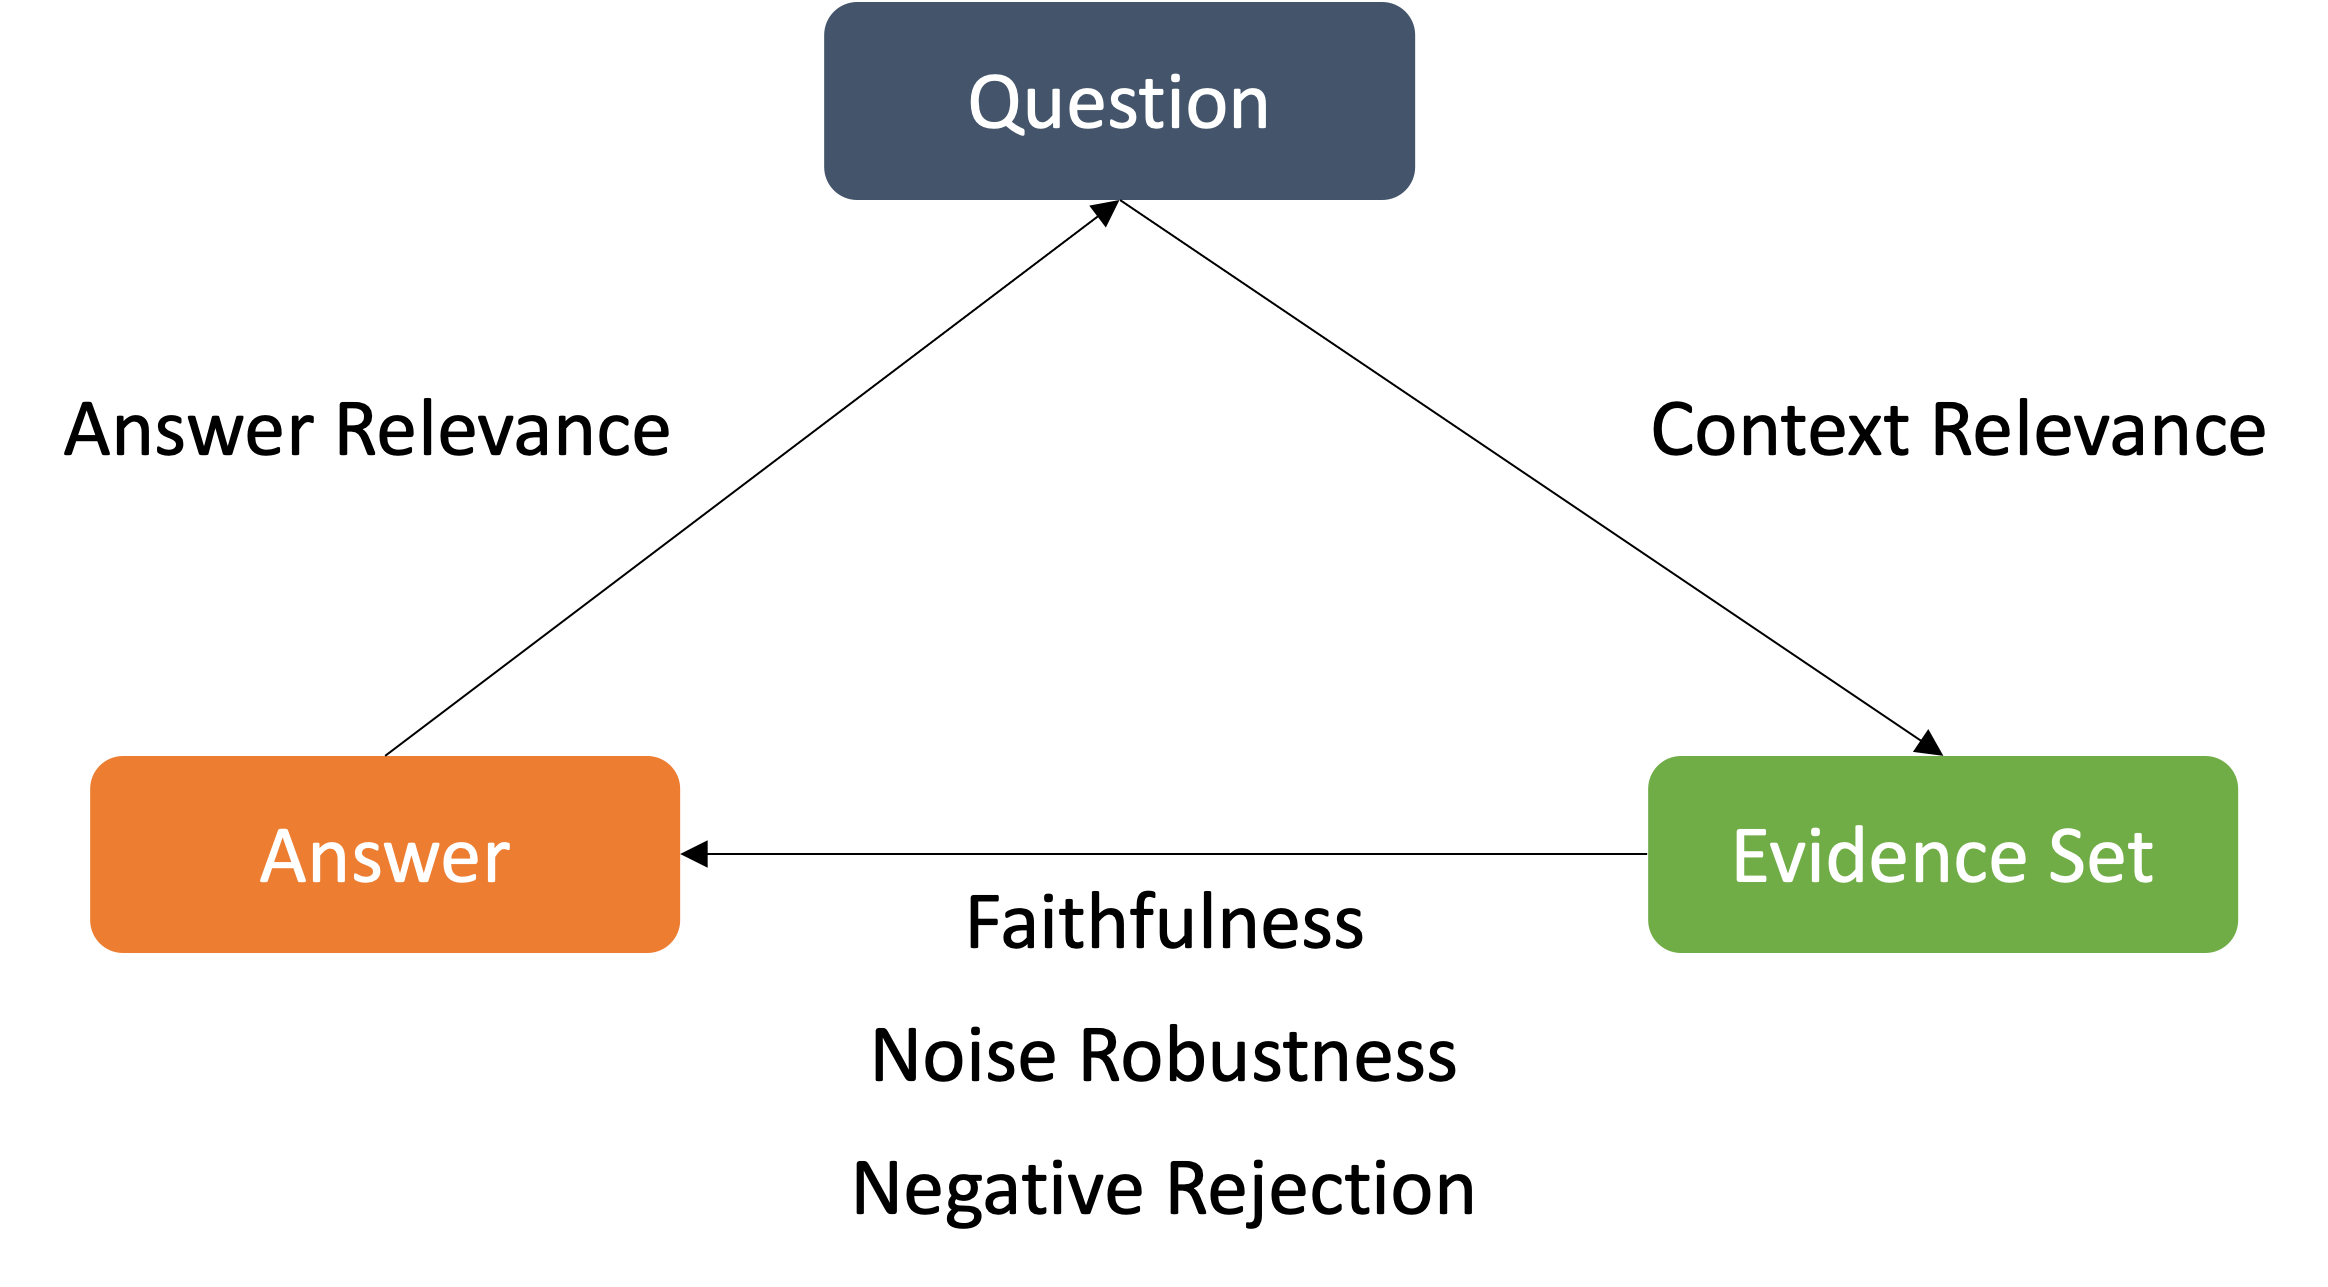
\includegraphics[width=\textwidth]{Grafiken/Evaluation_Dimensions_RAGAS_Turelens.png} 
    \caption{Adapted Evaluation Aspects and Components by TruLens [TruLens, 2024]}
  \end{figure}
  
\end{frame}

\begin{frame}{Evaluation Metrics \& Approaches}
  \begin{columns}[T] % Added [T] option for top alignment
    \begin{column}{.55\textwidth}
      {\color{unirot}Metrics}
      \begin{itemize}
        \item \textbf{Retriever:}
          \begin{itemize}
            \item Hit Rate 
            \item Mean Reciprocal Rank
          \end{itemize}
        \item \textbf{Reader:}
          \begin{itemize}
            \item BLEU-1
            \item ROUGE-L
            \item F1-BERTScore\footnotemark[8]
            \item Accuracy
            \begin{itemize}
              \item LLM-based
              \item Human-based
            \end{itemize}
          \end{itemize}
      \end{itemize}
    \end{column}
    \begin{column}{.45\textwidth}
      {\color{unirot}End-to-End Approach}
      \begin{enumerate}
        \item Human evaluator starts a context-dependent conversation.
        \item Conversation lasts for 4-10 turns.
        \item Post-conversation, RAG evaluation aspects are assessed turnwise using Knowledge Base, Evidence Set, and contextualized Query, including the \textit{Reason for Incorrectness}.
      \end{enumerate}
    \end{column}
  \end{columns}
\end{frame}

\subsection{Limitations}

\begin{frame}{Evaluation Limitations}

  \textbf{Limiting Factors for auto single component Evaluation:}
  \begin{itemize}
    \item LLM Performance
    \item Gold-Answer-Generation Performance
    \item Generated Question Usefulness
    \item Negative Rejection Evaluation
    \item BLUE and ROUGE Metrics
  \end{itemize}

  \bigskip

  \begin{block}{Conclusion}
    Auto evaluation suits extractive questions due to question-context-answer structure. New methods are needed for abstractive and complex questions.
  \end{block}
    
\end{frame}

\subsection{End-to-End Evaluation}


\begin{frame}{End-to-End Evaluation}

  \begin{columns}[T]
    \begin{column}{.5\textwidth}
      \begin{itemize}
        \item \alert<1>{Context Relevance}
        \item Faithfulness
        \item Noise Robustness
        \item Negative Rejection
        \item Answer Relevance
      \end{itemize}
    \end{column}

    \begin{column}{.5\textwidth}
      \centering

      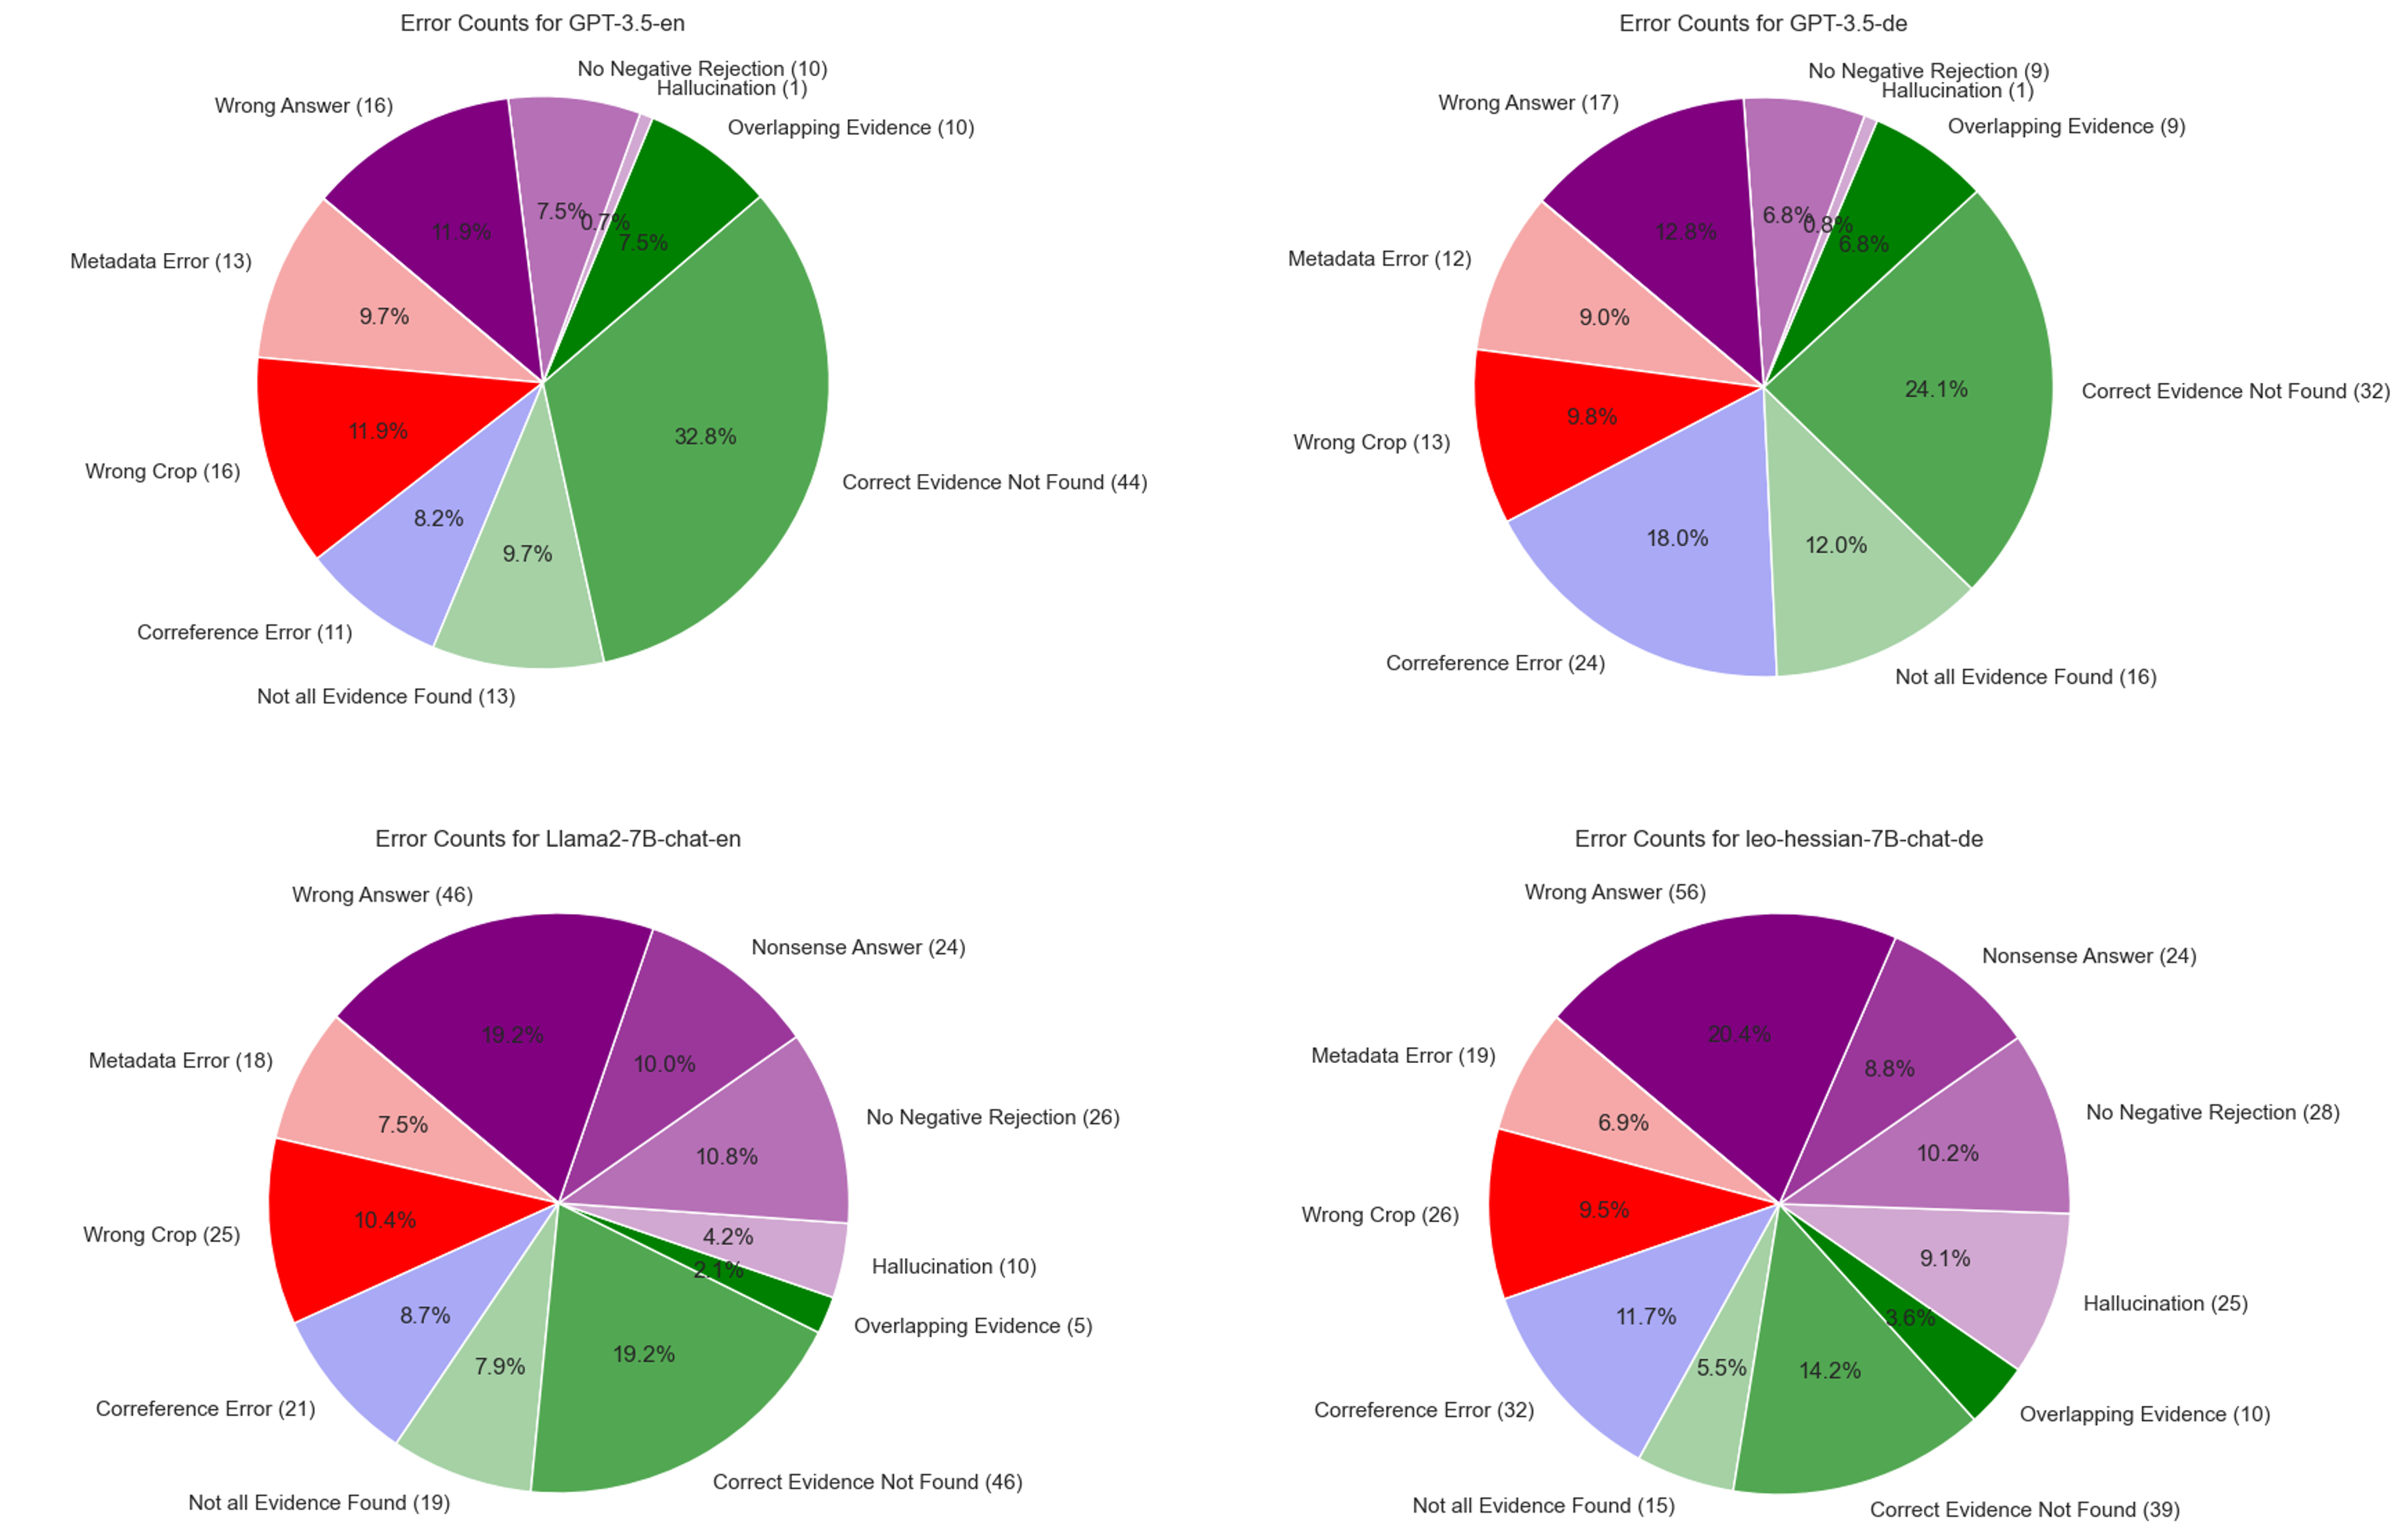
\includegraphics[width=0.9\textwidth]{Grafiken/Combined_Plots.png}
      \captionsetup{font={tiny}} % This line changes the caption font size
      \captionof{figure}{Reason for Incorrectness Distribution per Model}

      \resizebox{0.9\textwidth}{!}{% Add this line
        \begin{tabular}{lrr}
          \toprule
           & avg. Context Relevance & Count \\
          Question Type &  &  \\
          \midrule
          Abstract & 0.404040 & 99 \\
          Complex & 0.282051 & 39 \\
          Factoid & 0.492308 & 195 \\
          List & 0.833333 & 18 \\
          Yes/No & 0.428571 & 14 \\
          \bottomrule
        \end{tabular}
      }% And this line
      \captionof{table}{Average Context Relevance per Question Type}
      \label{tab:context-relevance-per-question-type}
    \end{column}

  \end{columns}

\end{frame}


\begin{frame}{End-to-End Evaluation}

  \begin{columns}[T]
    \begin{column}{.5\textwidth}
      \begin{itemize}
        \item \alert<1>{Context Relevance}
        \item Faithfulness
        \item Noise Robustness
        \item Negative Rejection
        \item Answer Relevance
      \end{itemize}
    \end{column}

    \begin{column}{.5\textwidth}
      \centering

      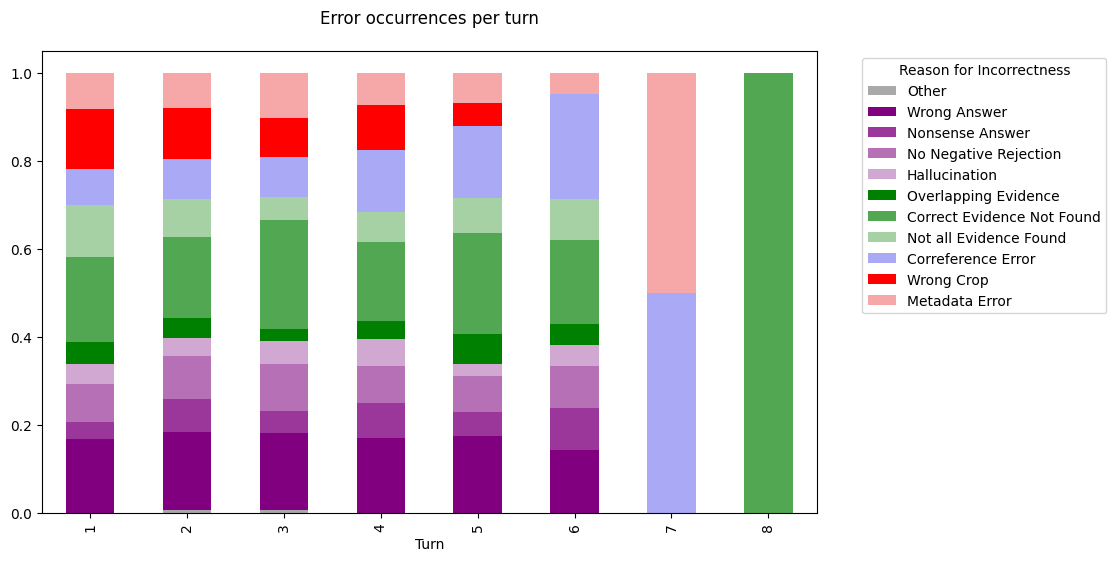
\includegraphics[width=0.9\textwidth]{Grafiken/Turns-Errors.png}
      \captionsetup{font={tiny}} % This line changes the caption font size
      \captionof{figure}{Reason for Incorrectness Distribution per Turn}
   \end{column}

  \end{columns}

\end{frame}


\begin{frame}{End-to-End Evaluation}
    \begin{itemize}
      \item Context Relevance
      \item \alert<1>{Faithfulness}
      \item Noise Robustness
      \item Negative Rejection
      \item Answer Relevance
    \end{itemize}

    \begin{table}
      \centering
      \resizebox{\textwidth}{!}{%
        \begin{tabular}{lrrrrrrr}
          \toprule
          & avg. Faithfullness & Count & avg. AR1* & Count & avg. AR\textgreater1** & Count & Negative Rejection Specificity\\
          Model Language &  &  &  &  &  &  &  \\
          \midrule
          GPT-3.5-de & 0.892 & 93 & 0.692 & 26 & 0.654 & 13 & 0.607 \\
          GPT-3.5-en & 0.908 & 98 & 0.550 & 20 & 0.613 & 8 & 0.826 \\
          Llama2-7B-chat-en & 0.726 & 95 & 0.395 & 19 & 0.373 & 15 & 0.128 \\
          leo-hessian-7B-chat-de & 0.620 & 92 & 0.300 & 23 & 0.200 & 24 & 0.467 \\
          \bottomrule
        \end{tabular}
      }
      \begin{tabular}{p{\textwidth}}
        {\raggedright\tiny * \textit{AR1} stands for \textit{Answer Relevance} where the \textit{Context Position = 1}\par}
        {\raggedright\tiny ** \textit{AR\textgreater1} stands for \textit{Answer Relevance} where the \textit{Context Position \textgreater 1}\par}
      \end{tabular}
      \vspace*{-5mm} % Adjust this value as needed
      \captionsetup{font={tiny}} % This line changes the caption font size
      \caption{Multiple Metrics per Model and Language}
      \label{tab:average-faithfullness-and-context-relevance-per-model-language}
    \end{table}

\end{frame}


\begin{frame}{End-to-End Evaluation}
  \begin{itemize}
    \item Context Relevance
    \item Faithfulness
    \item \alert<1>{Noise Robustness}
    \item Negative Rejection
    \item Answer Relevance
  \end{itemize}

  \begin{table}
    \centering
    \resizebox{\textwidth}{!}{%
      \begin{tabular}{lrrrrrrr}
        \toprule
        & avg. Faithfullness & Count & avg. AR1* & Count & avg. AR\textgreater1** & Count & Negative Rejection Specificity\\
        Model Language &  &  &  &  &  &  &  \\
        \midrule
        GPT-3.5-de & 0.892 & 93 & 0.692 & 26 & 0.654 & 13 & 0.607 \\
        GPT-3.5-en & 0.908 & 98 & 0.550 & 20 & 0.613 & 8 & 0.826 \\
        Llama2-7B-chat-en & 0.726 & 95 & 0.395 & 19 & 0.373 & 15 & 0.128 \\
        leo-hessian-7B-chat-de & 0.620 & 92 & 0.300 & 23 & 0.200 & 24 & 0.467 \\
        \bottomrule
      \end{tabular}
    }
    \begin{tabular}{p{\textwidth}}
      {\raggedright\tiny * \textit{AR1} stands for \textit{Answer Relevance} where the \textit{Context Position = 1}\par}
      {\raggedright\tiny ** \textit{AR\textgreater1} stands for \textit{Answer Relevance} where the \textit{Context Position \textgreater 1}\par}
    \end{tabular}
    \vspace*{-5mm} % Adjust this value as needed
    \captionsetup{font={tiny}} % This line changes the caption font size
    \caption{Multiple Metrics per Model and Language}
    \label{tab:average-faithfullness-and-context-relevance-per-model-language}
  \end{table}
\end{frame}


\begin{frame}{End-to-End Evaluation}
  \begin{itemize}
    \item Context Relevance
    \item Faithfulness
    \item Noise Robustness
    \item \alert<1>{Negative Rejection}
    \item Answer Relevance
  \end{itemize}

  \begin{table}
    \centering
    \resizebox{\textwidth}{!}{%
      \begin{tabular}{lrrrrrrr}
        \toprule
        & avg. Faithfullness & Count & avg. AR1* & Count & avg. AR\textgreater1** & Count & Negative Rejection Specificity\\
        Model Language &  &  &  &  &  &  &  \\
        \midrule
        GPT-3.5-de & 0.892 & 93 & 0.692 & 26 & 0.654 & 13 & 0.607 \\
        GPT-3.5-en & 0.908 & 98 & 0.550 & 20 & 0.613 & 8 & 0.826 \\
        Llama2-7B-chat-en & 0.726 & 95 & 0.395 & 19 & 0.373 & 15 & 0.128 \\
        leo-hessian-7B-chat-de & 0.620 & 92 & 0.300 & 23 & 0.200 & 24 & 0.467 \\
        \bottomrule
      \end{tabular}
    }
    \begin{tabular}{p{\textwidth}}
      {\raggedright\tiny * \textit{AR1} stands for \textit{Answer Relevance} where the \textit{Context Position = 1}\par}
      {\raggedright\tiny ** \textit{AR\textgreater1} stands for \textit{Answer Relevance} where the \textit{Context Position \textgreater 1}\par}
    \end{tabular}
    \vspace*{-5mm} % Adjust this value as needed
    \captionsetup{font={tiny}} % This line changes the caption font size
    \caption{Multiple Metrics per Model and Language}
    \label{tab:average-faithfullness-and-context-relevance-per-model-language}
  \end{table}

\end{frame}


\begin{frame}{End-to-End Evaluation}
  \begin{columns}[T]
    \begin{column}{.5\textwidth}
      \begin{itemize}
        \item Context Relevance
        \item Faithfulness
        \item Noise Robustness
        \item Negative Rejection
        \item \alert<1>{Answer Relevance}
      \end{itemize}
    \end{column}
    \begin{column}{.5\textwidth}
      \begin{table}[h]
        \centering
        \resizebox{\textwidth}{!}{%
        \begin{tabular}{lll}
          \toprule
          Model-Language         & Number of Error-free turns & avg. Answer Relevance \\
          \midrule
          GPT-3.5-de             & 14 (20.59 \%)*              & 0.7786                \\
          GPT-3.5-en             & 10 (17.54 \%)*              & 0.85                  \\
          Llama2-7B-chat-en      & 3 (3.37 \%)*                & 0.7333                \\
          leo-hessian-7B-chat-de & 8 (10.26 \%)*               & 0.825                 \\
          \bottomrule
          {\raggedright\footnotesize * The percentage compared to all turns}
        \end{tabular}%
        }
        \captionsetup{font=tiny}
        \caption{Error-free turns per Model and Language}
        \label{tab:correct-turns-per-model}
      \end{table}
    \end{column}
  \end{columns}

  \begin{table}[h]
    \centering
    \resizebox{\textwidth}{!}{%
    \begin{tabular}{lrrrrrrrrrrrrrr}
        \toprule
        & \multicolumn{2}{c}{GPT-3.5-de} & \multicolumn{2}{c}{GPT-3.5-en} & \multicolumn{2}{c}{Llama2-7B-chat-en} & \multicolumn{2}{c}{leo-hessian-7B-chat-de} \\
        Question Type & avg. AR* & Count & avg. AR* & Count & avg. AR* & Count & avg. AR* & Count \\
        \midrule
        Abstract & \textbf{0.478} & 18 & 0.421 & 14 & 0.200 & 31 & 0.258 & 12 \\
        Complex & \textbf{0.327} & 11 & 0.263 & 8 & 0.000 & 5 & 0.167 & 3 \\
        Factoid & 0.435 & 31 & \textbf{0.477} & 26 & 0.323 & 40 & 0.154 & 52 \\
        List & 0.550 & 4 & 0.467 & 6 & \textbf{0.600} & 2 & 0.225 & 4 \\
        Yes/No & \textbf{0.500} & 2 & 0.200 & 2 & 0.067 & 3 & 0.420 & 5 \\
        \bottomrule
    \end{tabular}%
    }
    {\raggedright\tiny * \textit{AR} stands for \textit{Answer Relevance}\par}
    \captionsetup{font=tiny}
    \caption{Answer Relevance per Model, Language and Question Type}
    \label{tab:answer-relevance-per-model}
  \end{table}
\end{frame}

\section[Conclusion]{Conclusion}


\begin{frame}{Conclusion}
  \begin{columns}[T]
    \begin{column}{.5\textwidth}
      {\color{unirot}Contributions}
      \begin{itemize}
        \item Decision map for ConRAG-System
        \item Operations-based extraction
        \item Approaches to improve reader and retriever
        \item Limitations of synthetic auto component-wise evaluation
        \item Evaluation approaches for end-to-end RAG evaluation
      \end{itemize}
    \end{column}
    \begin{column}{.5\textwidth}
      {\color{unirot}Future Work}
      \begin{itemize}
        \item Feasibility of ConQA Systems
        \item Constrained System Design
        \item Improving the Retriever
        \item PDF Data Extraction
      \end{itemize}
    \end{column}
  \end{columns}
\end{frame}


\section*{Backup}

\subsection*{Backup}

\begin{frame}{Backup - Model links}
  \tiny{
  \begin{enumerate}
    \item \url{https://github.com/dorianbrown/rank_bm25}
    \item \url{https://huggingface.co/cross-encoder/ms-marco-MiniLM-L-6-v2}
    \item \url{https://huggingface.co/cross-encoder/msmarco-MiniLM-L6-en-de-v1}
    \item \url{https://platform.openai.com/docs/models/embeddings}
    \item \url{https://platform.openai.com/docs/models/gpt-3-5}
    \item \url{https://huggingface.co/TheBloke/Llama-2-7b-Chat-GPTQ}
    \item \url{https://huggingface.co/TheBloke/leo-hessianai-7B-chat-GPTQ}
    \item \url{https://huggingface.co/spaces/evaluate-metric/bertscore}
  \end{enumerate}
  }
\end{frame}
% \section[Structure]{Page Structure}

% \subsection{Enumerations}


% \frame{
% \frametitle{Enumerations}

% \begin{itemize}
% \item Item
% \begin{itemize}
%   \item Subitem 1
%   \item Subitem 2
%   \item Subitem 3
% \end{itemize}
% \item Another main item
% \item And yet another one
% \begin{itemize}
%   \item \ldots with subitem
% \end{itemize}
% \end{itemize}
% } % END OF FRAME

% %----------------------------------------

% \frame{
% \frametitle{Enumerations / 2}

% \begin{itemize}
% \item Item
% \medskip
% \begin{itemize}
%   \item Subitem 1
%   \medskip
%   \item Subitem 2
%   \medskip
%   \item Subitem 3
% \end{itemize}
% \bigskip
% \item And another item
% \bigskip
% \item And yet another one
% \medskip
% \begin{itemize}
%   \item again with subitem
% \end{itemize}
% \end{itemize}
% } % END OF FRAME

% %----------------------------------------

% \frame[t]{
% \frametitle{Enumerations / 3}

% \begin{itemize}
% \item Main item with 3 subitems
% \begin{itemize}
%   \item[(a)] Subitem 1
%   \item[(b)] Subitem 2
%   \item[(c)] Subitem 3
% \end{itemize}
% \item And another item
% \item And yet another one
% \begin{itemize}
%   \item \ldots again with subitem 
% \end{itemize}
% \end{itemize}
% } % END OF FRAME

% %========================================

% \subsection{Rows}


% \frame{
% \frametitle{Rows}

% \begin{columns}[t]
% \begin{column}{.5\textwidth}
% {\color{unirot}Advantages}
% \begin{itemize}
%   \item There are many
%   \item and more
%   \item and even more
%   \item and a last advantage
% \end{itemize}
% \end{column}


% \begin{column}{.5\textwidth}
% {\color{unirot}Disadvantages} 
% \begin{itemize}
%   \item There is only one 
%   \item or two
% \end{itemize}
% \end{column}

% \end{columns}
% \vfill
% } % END OF FRAME

% %----------------------------------------

% \frame{
% \frametitle{Rows / 2}

% \begin{columns}[b]
% \begin{column}{.5\textwidth}
% {\color{unirot}Advantages}
% \begin{itemize}
%    \item There are many
%   \item and more
%   \item and even more
%   \item and a last advantage
% \end{itemize}
% \end{column}


% \begin{column}{.5\textwidth}
% {\color{unirot}Disadvantages} 
% \begin{itemize}
%   \item There is only one 
%   \item or two
% \end{itemize}
% \end{column}

% \end{columns}
% \vfill
% } % END OF FRAME

% %========================================

% \subsection{Blocks}


% \frame{
% \frametitle{Blocks}

% \begin{block}{\centering Definition of x}
% x is an important parameter for any type of text.
% \end{block}

% \medskip
% \begin{block}{\centering Steps}
% \begin{itemize}
%   \item[(1)] Practice
%   \item[(2)] Practice
%   \item[(3)] Practice
% \end{itemize}
% \end{block}

% \medskip
% \begin{block}{}
% \centering

% A block does not require a title.
% \end{block}

% } % END OF FRAME



% %========================================
% %========================================

% \section[Transitions]{Transitions  between Slides}

% \subsection{Simpel pause and the like}


% \frame{
% \frametitle{Enumerations}

% \begin{itemize}
% \item Main item
% \begin{itemize}
%   \item Subitem 1
%   \item Subitem 2
%   \item Subitem 3
% \end{itemize}
% \pause

% \item Another main item
% \pause

% \item And yet another one
% \begin{itemize}
%   \item again with subitem
%   \pause
%   \item and a second subitem
% \end{itemize}
% \end{itemize}
% } % END OF FRAME

% %----------------------------------------

% \frame{
% \frametitle{Enumerations / 2}

% \begin{itemize}
% \item Main item
% \begin{itemize}
%   \item<1> Subitem 1
%   \item<2-3> Subitem 2
%   \item<3-> Subitem 3
% \end{itemize}
% \item<4> Another main item
% \item<4-> And yet another one
% \begin{itemize}
%   \item<6-> again with subitem
%   \item<7> and a second subitem
% \end{itemize}
% \end{itemize}
% } % END OF FRAME

% %========================================

% \subsection{Overlays}

% \frame{
% \frametitle{Overlay of Images}
% \vspace*{-2ex}

% \begin{overprint}
% \onslide<1>
% \begin{figure}
% 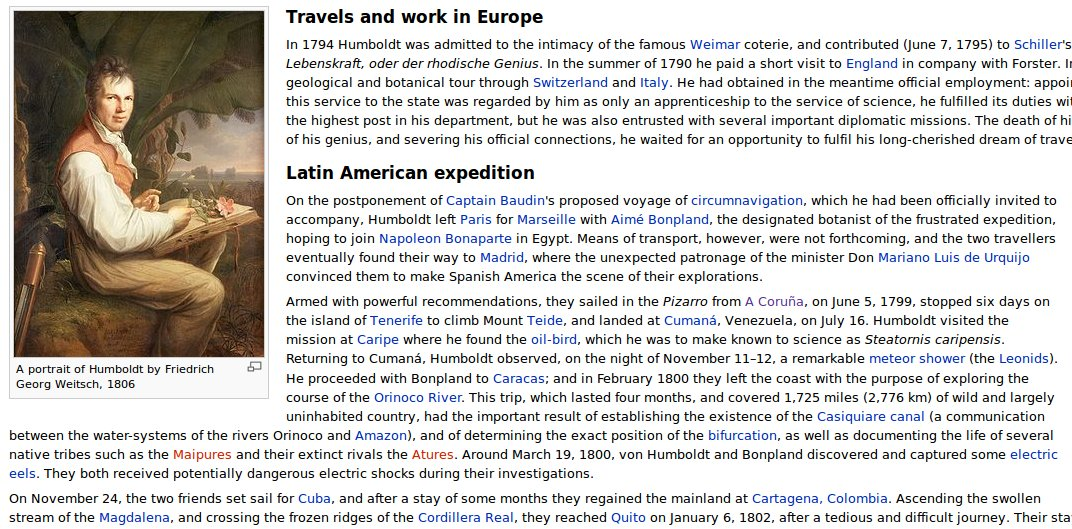
\includegraphics[width=\textwidth]{humboldt_wiki-blank.png} 
% \caption{AvH in Wikipedia, \textit{Source: URL}}
% \end{figure}

% \onslide<2>
% \begin{figure}
% 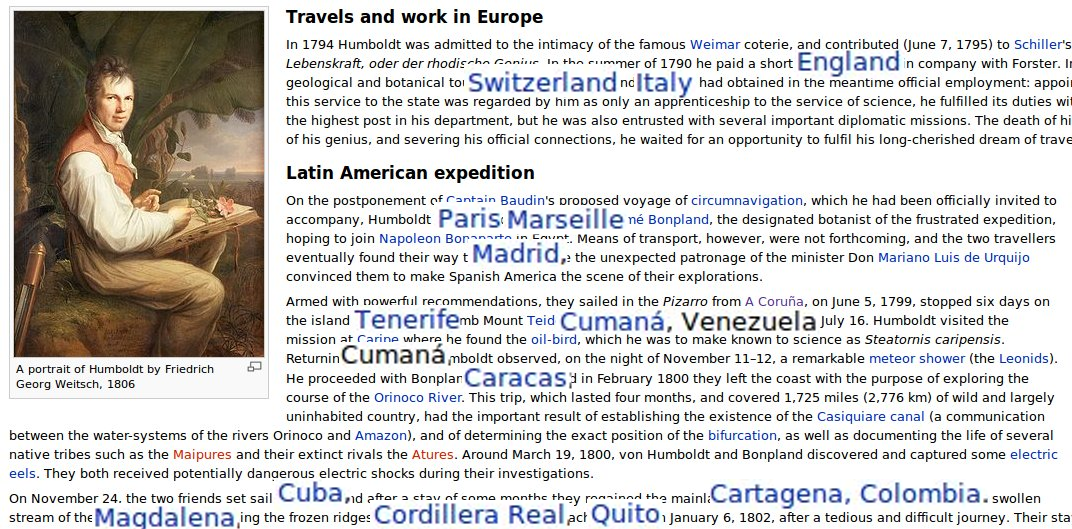
\includegraphics[width=\textwidth]{humboldt_wiki-locations.png} 
% \caption{AvH in Wikipedia, \textit{Source: URL}}
% \end{figure}

% \onslide<3>
% \begin{figure}
% 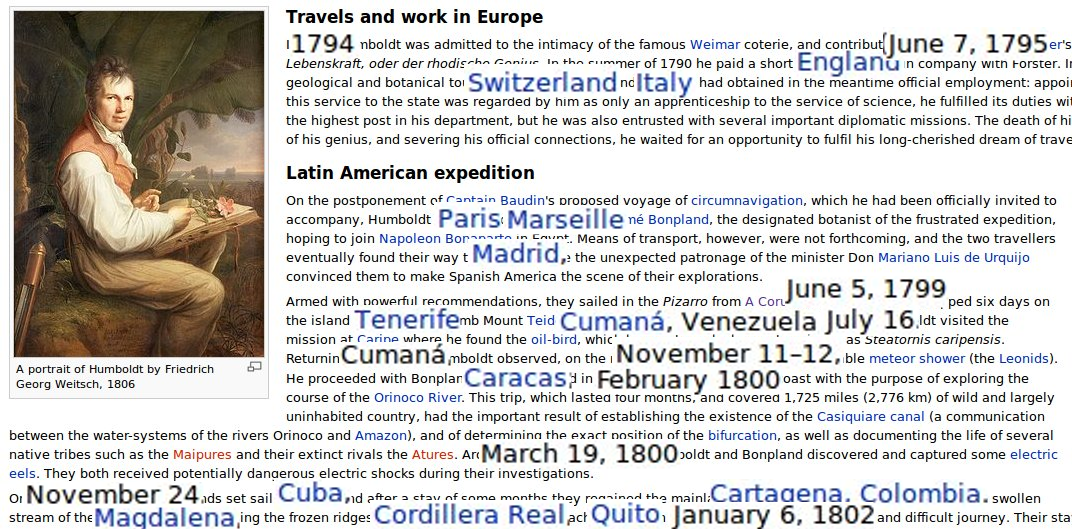
\includegraphics[width=\textwidth]{humboldt_wiki-locations-dates.png} 
% \caption{AvH in Wikipedia, \textit{Source: URL}}
% \end{figure}

% \onslide<4>
% \begin{figure}
% 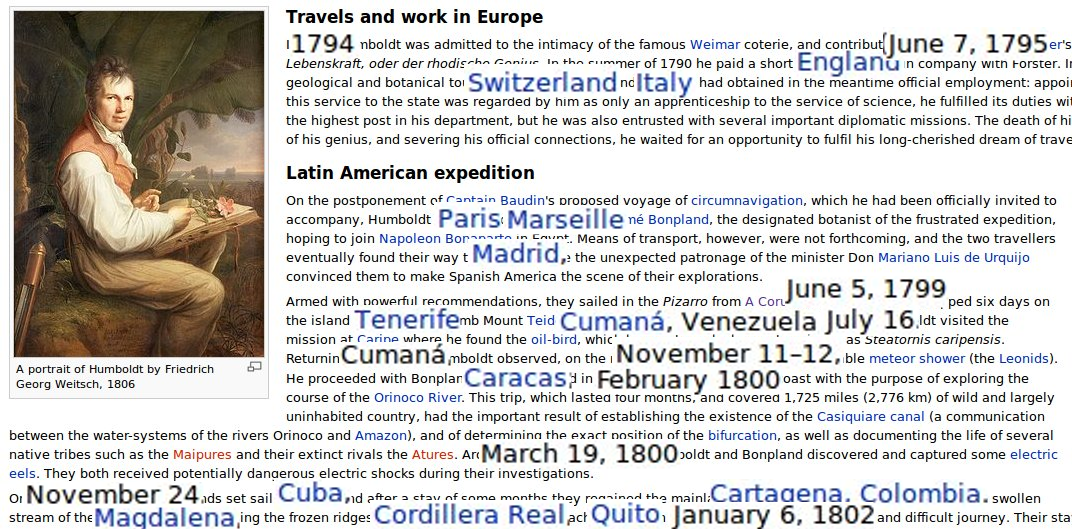
\includegraphics[width=\textwidth]{humboldt_wiki-locations-dates.png} 
% \caption{AvH in Wikipedia, \textit{Source: URL}}
% \end{figure}
% \vspace*{-5cm}
% \begin{block}{An the essence is \ldots}
% \textbf{There were many events in the life of AvH.}
% \end{block}

% \end{overprint}

% } % END OF FRAME

% %----------------------------------------



% \frame{\frametitle{Overlaying Details}
% \vspace*{-1ex}
% \begin{itemize}
% \item What are the issues?
% \begin{overprint}
% \onslide<1>
%   \begin{itemize}
%   \item Issue 1
%   \item Issue 2
%   \item Issue 3
%   \end{itemize}
% \onslide<2>
%   \begin{itemize}
%   \item Issue 1 \\
% \vspace*{-3ex}  
%   \begin{center}
% \includegraphics[width=.3\textwidth]{questions}
% \end{center}
%   \item Issue 2
%   \item Issue 3
%   \end{itemize}
% \onslide<3>
%   \begin{itemize}
%   \item Issue 1
%   \item Issue 2 \\
%   \begin{center}
%   \includegraphics[width=.3\textwidth]{questions}
%   \end{center}
%   \item Issue 3
%   \end{itemize}
% \onslide<4>
%   \begin{itemize}
%   \item Issue 1
%   \item Issue 2
%   \item Issue 3 \\
%   \begin{center}
%   \includegraphics[width=.3\textwidth]{questions}
%   \end{center}
%   \end{itemize}
% \end{overprint}
% \end{itemize}
% } % END OF FRAME



% %========================================
% %========================================

% \section{Accentuations}

% \subsection{Accentuations}

% %----------------------------------------

% \def\hilite<#1>{%
%   \temporal<#1>{\color{black}}{\color{unirot}}%
%                {\color{gray}}}
               
% %----------------------------------------

% \frame{
% \frametitle{Accentuating Parts of Text }

% \textbf{Source:} Beamer v3.0 Guide
% \bigskip

% \begin{Large}
% \begin{tabular}{|p{3.5cm}|}
% \hline
% \texttt{{\hilite<4>A}( Id,{ \hilite<2>X}, {\hilite<3>Y})} \\
% \texttt{B( Id, {\hilite<2>X}, {\hilite<3>Y})} \\ 
% \hline
% \end{tabular}
% \end{Large} 

% } % END OF FRAME

% %----------------------------------------

% \frame{
% \frametitle{Accentuating Parts of Text / 2}

% \textbf{Source:} Beamer v3.0 Guide

% \bigskip
% \begin{itemize}
% \item<1-2> \alert<1>{This is important}
% \item \alert<2-3>{Now this is important}
% \item \alert<3>{Now both are important}
% \item This is never important
% \end{itemize}

% } % END OF FRAME


% %========================================
% %========================================

% \section[More]{More Information}

% \subsection{More Information}

% \frame{
% \frametitle{Useful Beamer Tutorials}

% \begin{itemize}
% \item The Beamer class -- CTAN\\
% \url{http://ctan.math.utah.edu/ctan/tex-archive/macros/latex/contrib/beamer/doc/beameruserguide.pdf}
% \item ``A Beamer Tutorial in Beamer'' von Charles T. Batts \\
% \url{https://www.uncg.edu/cmp/reu/presentations/Charles\%20Batts\%20-\%20Beamer\%20Tutorial.pdf}
% %\texttt{http://www.uncg.edu/cmp/reu/presentations/Charles \\ \%20Batts\%20-\%20Beamer\%20Tutorial.pdf}
% \medskip
% \item The Beamer class for \LaTeX\\
% \url{http://www.mathematik.uni-leipzig.de/~hellmund/LaTeX/beamer2.pdf}
% \medskip
% \item Beamer Theme Matrix \\
% \texttt{http://www.hartwork.org/beamer-theme-matrix/}
% \end{itemize}

% }

% %----------------------------------------

% \frame{\frametitle{Questions}
% \begin{figure}
% \includegraphics[width=.8\textwidth]{questions} 
% \end{figure}
% \vspace*{-3.3cm}\begin{center}\begin{LARGE}\textbf{Questions}\end{LARGE}\end{center}

% \vspace*{2cm}
% }

\end{document}
